\def\GraphicsFolder{chapters/superconducting-instability/pictures}
\chapter{Superconducting phase}\label{chap:sc}

In this chapter, we study the translationally invariant superconducting (SC) phase. We observe various effects: bare bands shrinking, insurgence of mixed-symmetry superconductivity and nematicity.

This chapter is organised as follows. In Sec.~\ref{sec:sc-phase-theory} we present the translationally invariant superconducting phase and its symmetries. In Sec.~\ref{sec:sc-hf-hfps} we report the HF approximation to the EHM hamiltonian in the normal phase, the self-consistency equations and two constraints for the various HFPs.
In Sec.~\ref{sec:sc-numeric} we present the result of numeric simulations.

The analytical computations for the SC phase are almost identical to the ones carried out for the AF phase. For the sake of conciseness, in this section we limit to reporting the essential result, while the entire derivation is moved to App.~\ref{app:sc-hf-hamiltonian}.

\section{The SC phase and its symmetries}\label{sec:sc-phase-theory}

The translationally invariant SC phase is described by the SSB
\[
	\mathrm{U}^z(1) \SSB 0 \, , \\
\]
as we discussed in Sec.~\ref{sec:ehm-sym-break}. In the SC phase, products of two creation operators can be non-zero,
\[
	\big\langle
	\hat c_{i\sigma}^\dagger \hat c_{j\sigma'}^\dagger \rangle \neq 0 \, ,
\]
because charge is not conserved. We discussed this fact in Sec.~\ref{sec:ehm-sym-break}, when we proved that EVs of products of two creation operators are zero when charge is conserved. The above inequality has a precise meaning: adding two electrons to the ground state produces a state with a finite overlap with the ground state itself. In BCS theory, this is interpreted with the appearance of pairs of electrons bound together by an attractive interaction, i.e. Cooper pairs \cite{grosso2014solid,coleman2015introduction}.

Cooper pairs are composite quantum objects, with spatial and spin structure. Being couples of electrons, they obey antisymmetry rules under internal exchange, and their total spin follows the composition rules of spin algebras
\[
	\frac 1 2 \otimes \frac 1 2 = 0 \oplus 1 \, ,
\]
which means that two $\mathfrak{su}(2)$ algebras are composed into a singlet and a triplet. The first is anti-symmetric under spin exchange; the second is symmetric. Hence, we can distinguish two Cooper pairing channels:
\begin{enumerate}
	\item Singlet, with total spin equal to $0$. In this channel, the Cooper pairs must exhibit spatial inversion symmetry.
	\item Triplet, with total spin equal to $1$. In this channel, the Cooper pairs must exhibit spatial inversion anti-symmetry.
\end{enumerate}
This concept is summarised in Tab.~\ref{tab:sc-pairings-symmetry-structures}. We can choose to restrict to just one of these pairing channels. This provides specific symmetry selection rules on the superconducting gap function harmonics. In this thesis, we restrict to the singlet channel.

\begin{table}
	\centering
	\begin{tabular}{c c}
		\textbf{Spatial structure of Cooper pairs} & \textbf{Pairing channel} \\
		\midrule
		Inversion symmetric & Singlet pairing \\
		Inversion anti-symmetric & Triplet pairing \\
		\midrule
	\end{tabular}
	\caption{Relation between the spatial inversion (intended as $(x,y) \to (-x,-y)$) symmetry properties and the pairing channel for Cooper pairs.}
	\label{tab:sc-pairings-symmetry-structures}
\end{table}

As we did previously, we also allow for breaking of rotational symmetry,
\[
	\mathrm{C}_4 \SSB \mathrm{C}_2 \, .
\]
We will observe the breaking of planar rotational symmetry in the SC phase.

\section{The HF hamiltonian and the variational parameters in the SC phase}\label{sec:sc-hf-hfps}

In this section, we summarise the computations carried out in App.~\ref{app:sc-hf-hamiltonian} and report the final form of the HF hamiltonian. We define the operators
\begin{align}
	\hat n_{\mathbf{k}\sigma} &\equiv \hat c_{\mathbf{k}\sigma}^\dagger \hat c_{\mathbf{k}\sigma} \, , \label{eq:sc-ehm-n-def} \\
	\hat \phi_\mathbf{k} &\equiv \hat c_{-\mathbf{k}\downarrow} \hat c_{\mathbf{k}\uparrow} \, , \label{eq:sc-ehm-phi-def}
\end{align}
and their expectation values (EVs),
\begin{align}
	u_{\mathbf{k}\sigma} &\equiv \langle
	\hat n_{\mathbf{k}\sigma}
	\rangle \, , \label{eq:sc-uqsigma-def} \\
	w_\mathbf{k} &\equiv \langle
	\hat \phi_\mathbf{k}^\dagger
	\rangle \, . \label{eq:sc-wq-def}
\end{align}
The breaking of charge conservation, namely $\mathrm{U}^z(1)$ symmetry, allows $w_\mathbf{k}$ to become non-zero. Instead, for a phase which preserves $\mathrm{U}^z(1)$, $w_\mathbf{k}$ is identically zero.

Using the functions of Tab.~\ref{tab:x-wave-reciprocal-factors}, we define the harmonics
\begin{align}
	u^{(\gamma)}_\sigma &\equiv \frac{1}{L_x L_y} \sum_{\mathbf{k}\in\mathrm{BZ}} \varphi_\mathbf{k}^{(\gamma)} u_{\mathbf{k}\sigma} \, , \label{eq:sc-ugamma-harmonics} \\
	w^{(\gamma)} &\equiv \frac{1}{L_x L_y} \sum_{\mathbf{k}\in\mathrm{BZ}} \varphi_\mathbf{k}^{(\gamma)} w_\mathbf{k} \, . \label{eq:sc-wgamma-harmonics}
\end{align}
As was for the AF phase, these harmonics are HFPs in the SC phase and must be determined self-consistently. Eqs.~\eqref{eq:sc-ugamma-harmonics} and \eqref{eq:sc-wgamma-harmonics}.

%\section{The SC phase in the conventional HM}\label{sec:sc-hm}
%
%The conventional HM is given by $\hat H_t + \hat H_U$, thus its unique two-body interaction is the local repulsion. In this section, we study superconductivity in the conventional HM, and prove that it is impossible at HF level.
%
%\subsection{Derivation of the HF hamiltonian }\label{subsec:sc-hm-derivation}
%
%Following Tab.~\ref{tab:HU-sel-rules} and Eqs.~\eqref{eq:mft-HU}, \eqref{eq:mft-HV}, we know the local repulsion decomposes in Hartree and Cooper channels,
%\[
%\begin{aligned}
%	\hat H_U &= U \sum_{\mathbf{r}\in\mathcal{L}} \hat n_{\mathbf{r}\uparrow} \hat n_{\mathbf{r}\downarrow} \\
%	&\HFsimeq U \sum_{\mathbf{r}\in\mathcal{L}} \Big(
%	\hat c_{\mathbf{r}\uparrow}^\dagger \hat c_{\mathbf{r}\uparrow} \big\langle \hat c_{\mathbf{r}\downarrow}^\dagger \hat c_{\mathbf{r}\downarrow} \big\rangle + \big\langle \hat c_{\mathbf{r}\uparrow}^\dagger \hat c_{\mathbf{r}\uparrow} \big\rangle \hat c_{\mathbf{r}\downarrow}^\dagger \hat c_{\mathbf{r}\downarrow} - \big\langle \hat c_{\mathbf{r}\uparrow}^\dagger \hat c_{\mathbf{r}\uparrow} \big\rangle  \big\langle \hat c_{\mathbf{r}\downarrow}^\dagger \hat c_{\mathbf{r}\downarrow} \big\rangle &&(\text{Hartree}) \\
%	&\phantom{\HFsimeq \sum_{{\mathbf{r}\uparrow}\neq{\mathbf{r}\downarrow}} V_{{\mathbf{r}\uparrow}{\mathbf{r}\downarrow}}}
%	+ \hat c_{\mathbf{r}\uparrow}^\dagger \hat c_{\mathbf{r}\downarrow}^\dagger \big\langle \hat c_{\mathbf{r}\downarrow} \hat c_{\mathbf{r}\uparrow} \big\rangle + \big\langle \hat c_{\mathbf{r}\uparrow}^\dagger \hat c_{\mathbf{r}\downarrow}^\dagger \big\rangle \hat c_{\mathbf{r}\downarrow} \hat c_{\mathbf{r}\uparrow} - \big\langle \hat c_{\mathbf{r}\uparrow}^\dagger \hat c_{\mathbf{r}\downarrow}^\dagger \big\rangle  \big\langle \hat c_{\mathbf{r}\downarrow} \hat c_{\mathbf{r}\uparrow} \big\rangle
%	\Big) \, , &&(\text{Cooper})
%\end{aligned}
%\]
%while the Fock channel is identically zero. We deal with each channel separately.
%
%\paragraph{Local Hartree terms.}
%
%For the Hartree channel, being the density uniform across sites, we can re-use the entirety of Sec.~\ref{subsec:normal-hartree-mu} for the normal phase. Substituting Eq.~\eqref{eq:sc-<n_i>}, we get the approximation of Eq.~\eqref{eq:normal-HU-hartree-approx},
%\begin{equation}\label{eq:sc-HU-hartree-approx}
%	\hat H_U \HFsimeq nU \times \hat N - E_{\mathrm{H},U}^{(\mathrm{SC})} + \text{(Cooper channel)} \, ,
%\end{equation}
%thus chemical potential renormalisation,
%\begin{equation}\label{eq:sc-mu-shift-int}
%	\tilde{\mu} = \mu - nU
%\end{equation}
%is present also in the SC phase. Note that $\tilde{\mu}$ will be renormalised again, later, and we will redefine it accordingly. The contraction energy is the same of Eq.~\eqref{eq:normal-HU-hartree-Ec}
%\begin{equation}\label{eq:sc-HU-hartree-Ec}
%	E_{\mathrm{H},U}^{(\mathrm{SC})} = L_x L_y \times n^2 U \, .
%\end{equation}
%
%\paragraph{Local Cooper terms.}
%
%We move to reciprocal space, through the transformation of Eq.~\eqref{eq:HU-fourier}. Consider the Cooper channel of Eq.~\eqref{eq:mft-HU}. In reciprocal space we get:
%\begin{multline}
%	\hat H_U \HFsimeq \text{(Hartree channel)} + \frac{U}{L_x L_y}
%	\sum_{\mathbf{K}, \mathbf{k}, \mathbf{k}'} \Big(
%	\big\langle
%	\hat c_{\mathbf{K}+\mathbf{k} \uparrow}^\dagger \hat c_{\mathbf{K}-\mathbf{k} \downarrow}^\dagger
%	\big\rangle \hat c_{\mathbf{K}-\mathbf{k}' \downarrow} \hat c_{\mathbf{K}+\mathbf{k}' \uparrow} \\
%	+ \hat c_{\mathbf{K}+\mathbf{k} \uparrow}^\dagger \hat c_{\mathbf{K}-\mathbf{k} \downarrow}^\dagger \big\langle
%	\hat c_{\mathbf{K}-\mathbf{k}' \downarrow} \hat c_{\mathbf{K}+\mathbf{k}' \uparrow} 
%	\big\rangle - \big\langle
%	\hat c_{\mathbf{K}+\mathbf{k} \uparrow}^\dagger \hat c_{\mathbf{K}-\mathbf{k} \downarrow}^\dagger
%	\big\rangle \big\langle 
%	\hat c_{\mathbf{K}-\mathbf{k}' \downarrow} \hat c_{\mathbf{K}+\mathbf{k}' \uparrow}
%	\big\rangle
%	\Big) \, . \label{eq:sc-mft-HU}
%\end{multline}
%We are not breaking translational invariance, therefore,
%\begin{equation}\label{eq:sc-<cc>=delta}
%	\big\langle \hat c_{\mathbf{k}\sigma}^\dagger \hat c_{\mathbf{k}'\sigma'}^\dagger \big\rangle = \big\langle \hat c_{\mathbf{k}\sigma}^\dagger \hat c_{\mathbf{k}\sigma'}^\dagger \big\rangle \delta_{\mathbf{k}=-\mathbf{k}'} \, .
%\end{equation}
%
%\begin{tabproof}[Proof of Eq.~\eqref{eq:sc-<cc>=delta}]
%	Consider the EV
%	\[
%		\big\langle \hat c_{\mathbf{k}\sigma}^\dagger \hat c_{\mathbf{k}'\sigma'}^\dagger \big\rangle \, ,
%	\]
%	for two momenta $\mathbf{k}$, $\mathbf{k}'$. Moving to real space via an $\mathcal{F}$-transform, we get
%	\[
%		\big\langle \hat c_{\mathbf{k}\sigma}^\dagger \hat c_{\mathbf{k}'\sigma'}^\dagger \big\rangle \Feq \frac{1}{L_x L_y} \sum_{\mathbf{r} \in \mathcal{L}} \sum_{\mathbf{r}' \in \mathcal{L}} e^{-i \left(\mathbf{k} \cdot \mathbf{r} + \mathbf{k}' \cdot \mathbf{r}'\right)} \big\langle \hat c_{\mathbf{r}\sigma}^\dagger \hat c_{\mathbf{r}'\sigma'}^\dagger \big\rangle \, ,
%	\]
%	where we used the convention of Eq.~\eqref{eq:fourier-convention}. Let now $\mathbf{r} \equiv \mathbf{r}$ and $\Delta \mathbf{r} \equiv \mathbf{r} - \mathbf{r}'$. Translational invariance implies that the function
%	\[
%		g(\Delta \mathbf{r},\sigma,\sigma') = \big\langle \hat c_{\mathbf{r}\sigma}^\dagger \hat c_{\mathbf{r}+\Delta\mathbf{r}\sigma'}^\dagger \big\rangle
%	\]
%	is independent of $\mathbf{r}$. Thus, we have:
%	\[
%	\begin{aligned}
%		\big\langle \hat c_{\mathbf{k}\sigma}^\dagger \hat c_{\mathbf{k}'\sigma'}^\dagger \big\rangle &\Feq \sum_{\Delta\mathbf{r} \in \mathcal{L}} e^{-i \mathbf{k}' \cdot \Delta\mathbf{r}} g(\Delta \mathbf{r},\sigma,\sigma') \frac{1}{L_x L_y} \sum_{\mathbf{r} \in \mathcal{L}} e^{-i \left(\mathbf{k} + \mathbf{k}'\right) \cdot \mathbf{r}} \\
%		&= \sum_{\Delta\mathbf{r} \in \mathcal{L}} e^{-i \mathbf{k}' \cdot \Delta\mathbf{r}} g(\Delta \mathbf{r},\sigma,\sigma') \delta_{\mathbf{k}=\mathbf{k}'} \, ,
%	\end{aligned}
%	\]
%	where we used the identity of Eq.~\eqref{eq:ehm-delta}. Then, the above EV vanishes for $\mathbf{k}\neq\mathbf{k}'$. This proves Eq.~\eqref{eq:sc-<cc>=delta}.
%	
%\end{tabproof}
%
%Using Eq.~\eqref{eq:sc-<cc>=delta} in Eq.~\eqref{eq:sc-mft-HU}, only $\mathbf{K}=\mathbf{0}$ gives a non-zero contribution, and we obtain
%\begin{equation}\label{eq:sc-HU-cooper-approx}
%	\hat H_U \HFsimeq \text{(Hartree channel)} - \sum_{\mathbf{k}\in\mathrm{BZ}} \left(
%	\Delta^{(s)} \hat \phi_\mathbf{k} + 
%	\Delta^{(s)*} \hat \phi_\mathbf{k}^\dagger
%	\right) - E_{\mathrm{C},U}^{(\mathrm{SC})} \, ,
%\end{equation}
%where we defined
%\begin{equation}\label{eq:sc-Delta^s}
%	\Delta^{(s)} \equiv -U w^{(s)} \, ,
%\end{equation}
%and the contraction energy is given by
%\begin{equation}\label{eq:sc-HU-hartree-Ec-implicit}
%	E_{\mathrm{C},U}^{(\mathrm{SC})} = - \frac{U}{L_x L_y}
%	\sum_{\mathbf{k}, \mathbf{k}'} \big\langle
%	\hat \phi_\mathbf{k}^\dagger
%	\big\rangle \big\langle 
%	\hat \phi_{\mathbf{k}'}
%	\big\rangle \, .
%\end{equation}
%
%\begin{tabproof}[Proof of Eq.~\eqref{eq:sc-HU-cooper-approx}: HF approximation of $\hat H_U$ in Cooper channel]
%	
%	Using Eqs.~\eqref{eq:sc-ehm-phi-def}, \eqref{eq:sc-mft-HU} and \eqref{eq:sc-<cc>=delta}, we obtain
%	\begin{equation}\label{eq:sc-HU-<phi>-phi}
%		\hat H_U \HFsimeq \text{(Hartree channel)} + \frac{U}{L_x L_y} \sum_{\mathbf{k},\mathbf{k}'} \left(
%		\big\langle
%		\hat \phi_\mathbf{k}^\dagger
%		\big\rangle \hat \phi_{\mathbf{k}'} + 
%		\hat \phi_\mathbf{k}^\dagger \big\langle
%		\hat \phi_{\mathbf{k}'}
%		\big\rangle
%		\right) - E_{\mathrm{C},U}^{(\mathrm{SC})} \, ,
%	\end{equation}
%	From Eq.~\eqref{eq:sc-wq-def}, we have
%	\begin{multline*}
%		\hat H_U \HFsimeq \text{(Hartree channel)} + \left(
%			\frac{1}{L_x L_y} \sum_{\mathbf{k}\in\mathrm{BZ}} w_\mathbf{k}
%		\right) \times U \sum_{\mathbf{k}'\in\mathrm{BZ}} \hat \phi_{\mathbf{k}'} \\
%		+  \left(
%		\frac{1}{L_x L_y} \sum_{\mathbf{k}'\in\mathrm{BZ}} w_{\mathbf{k}'}^*
%		\right) \times U \sum_{\mathbf{k}\in\mathrm{BZ}} \hat \phi_\mathbf{k}^\dagger \, .
%	\end{multline*}
%	Therefore, from Eq.~\eqref{eq:sc-wgamma-harmonics}, we see that the parenthesised terms coincide, respectively, with $w^{(s)}$ and $w^{(s)*}$. Applying Eq.~\eqref{eq:sc-Delta^s}, we obtain Eq.~\eqref{eq:sc-HU-cooper-approx}.	
%\end{tabproof}
%
%The contraction energy of Eq.~\eqref{eq:sc-HU-hartree-Ec-implicit} reduces to
%\begin{equation}\label{eq:sc-HU-cooper-Ec}
%	E_{\mathrm{C},U}^{(\mathrm{SC})}=L_x L_y \times U \big| w^{(s)} \big|^2 \, .
%\end{equation}
%
%\begin{tabproof}[Proof of Eq.~\eqref{eq:sc-HU-cooper-Ec}: local Cooper contraction energy]
%	
%	Consider Eq.~\eqref{eq:sc-HU-hartree-Ec-implicit}. Substituting Eqs.~\eqref{eq:sc-wq-def}, \eqref{eq:sc-wgamma-harmonics} we get:
%	\begin{align}
%		E_{\mathrm{C},U}^{(\mathrm{SC})} &= L_x L_y \times U \left(\frac{1}{L_x L_y} \sum_{\mathbf{k}\in\mathrm{BZ}} w_\mathbf{k}^*\right) \left(\frac{1}{L_x L_y} \sum_{\mathbf{k}'\in\mathrm{BZ}} w_{\mathbf{k}'}\right) \\
%		&= L_x L_y \times U \big| w^{(s)} \big|^2 \, , \label{eq:sc-cooper-U-contraction-energy}
%	\end{align}
%	which proves Eq.~\eqref{eq:sc-HU-cooper-Ec}.
%\end{tabproof}
%
%In general, $\Delta^{(s)}$ as defined in Eq.~\eqref{eq:sc-Delta^s} is a complex number. However, we can always choose $\Delta^{(s)}$ as purely real. This is due to the fact that the hamiltonian is gauge-invariant. Indeed, if we set in Eq.~\eqref{eq:gauge-symmetry}
%\begin{equation}\label{eq:sc-gauge-ws-real}
%	\eta \equiv -\frac{\arg w^{(s)}}{2} \, ,
%\end{equation}
%we have $\Delta^{(s)} \in \mathbb{R}$.
%
%\begin{tabproof}[Choosing the gauge of Eq.~\eqref{eq:sc-gauge-ws-real}, we obtain a real gap]
%	Inserting Eq.~\eqref{eq:sc-gauge-ws-real} in Eq.~\eqref{eq:gauge-symmetry}, we obtain
%	\[
%		\hat c_{\mathbf{k}\sigma}^\dagger 
%		\quad\to\quad 
%		e^{- i\arg w^{(s)}/2} \hat c_{\mathbf{k}\sigma}^\dagger \, .
%	\]
%	Therefore,
%	\[
%		\hat \phi_\mathbf{k}^\dagger
%		\quad\to\quad 
%		\hat \phi_\mathbf{k}^\dagger e^{- i\arg w^{(s)}} 
%		\quad\implies\quad
%		w_\mathbf{k}
%		\quad\to\quad 
%		w_\mathbf{k} e^{- i\arg w^{(s)}} 
%		\, ,
%	\]
%	where we used Eq.~\eqref{eq:sc-wq-def}. It follows, from Eq.~\eqref{eq:sc-wgamma-harmonics},
%	\[
%		w^{(s)} \quad\to\quad w^{(s)} e^{- i\arg w^{(s)}} \, .
%	\]
%	For any complex number $z$, we have $z e^{-i \arg z} \in \mathbb{R}$. Then, $w^{(s)}$ is purely real under this gauge transform, and so is $\Delta^{(s)}$.
%\end{tabproof}
%
%\subsection{Diagonalisation of the HF hamiltonian}\label{subsec:sc-hm-diagonalisation}
%
%We proceed here as we did for the AF phase in Sec.~\ref{subsec:af-hm-diagonalisation}. We start by giving a matrix representation of the approximated hamiltonian, then map it to a pseudospin problem and finally specify how to diagonalise it to retrieve its ground state.
%
%\paragraph{Matrix representation.}
%
%Let $\Delta_\mathbf{k} = \Delta^{(s)}$. The HM gran-canonical hamiltonian is given by $\hat H_t + \hat H_U - \mu \hat N$. Its HF approximation for the SC phase can be written as
%\begin{equation}\label{eq:sc-HM-hk}
%	\hat H_t + \hat H_U - \mu \hat N \HFsimeq \sum_{\mathbf{k} \in \mathrm{BZ}} \sum_\sigma \hat \Phi_\mathbf{k}^\dagger h_\mathbf{k} \hat \Phi_\mathbf{k} + E_\mathrm{a}^{(\mathrm{SC})} - \left(
%	E_{\mathrm{H},U}^{(\mathrm{SC})} + E_{\mathrm{C},U}^{(\mathrm{SC})}
%	\right) \, ,
%\end{equation}
%where we defined the $2 \times 2$ matrix:
%\begin{equation}\label{eq:sc-hk}
%	h_\mathbf{k} \equiv \begin{bmatrix}
%		\xi_\mathbf{k} & -\Delta_\mathbf{k}^* \\
%		-\Delta_\mathbf{k} & - \xi_\mathbf{k}
%	\end{bmatrix}
%	\qq{with}
%	\xi_\mathbf{k} \equiv \epsilon_\mathbf{k} - \tilde{\mu} \, .
%\end{equation}
%In Eq.~\eqref{eq:sc-HM-hk}, we defined the Nambu spinors
%\begin{equation}\label{eq:sc-Phi-def}
%	\hat \Phi_\mathbf{k} \equiv \begin{bmatrix}
%		\hat c_{\mathbf{k}\uparrow} \\
%		\hat c_{-\mathbf{k}\downarrow}^\dagger
%	\end{bmatrix} \, ,
%\end{equation}
%and the ``anticommutation energy'' $E_\mathrm{a}^{(\mathrm{SC})}$,
%\begin{equation}\label{eq:sc-anticommutation-energy}
%	E_\mathrm{a}^{(\mathrm{SC})} \equiv \sum_{\mathbf{k}\in\mathrm{BZ}} \xi_\mathbf{k} \, .
%\end{equation}
%
%\begin{tabproof}[Proof of Eq.~\eqref{eq:sc-HM-hk}]
%
%	Summing Eq.~\eqref{eq:Ht-Fourier} and Eq.~\eqref{eq:sc-HU-cooper-approx}, we obtain
%	\begin{multline}
%		\hat H_t + \hat H_U \HFsimeq \sum_{\mathbf{k} \in \mathrm{BZ}} \sum_\sigma \epsilon_{\mathbf{k}\sigma}
%		\hat c_{\mathbf{k}\sigma}^\dagger \hat c_{\mathbf{k}\sigma} \\
%		- \sum_{\mathbf{k}\in\mathrm{BZ}} \left(
%		\Delta^{(s)} \hat \phi_\mathbf{k} + 
%		\Delta^{(s)*} \hat \phi_\mathbf{k}^\dagger
%		\right) + nU \times \hat N - \left(
%		E_{\mathrm{H},U}^{(\mathrm{SC})} + E_{\mathrm{C},U}^{(\mathrm{SC})}
%		\right) \, .
%		\label{eq:sc-hm-mft-h} 
%	\end{multline}
%	Inversion symmetry is not broken, then $\xi_\mathbf{k} = \xi_{-\mathbf{k}}$. Using Fermi anticommutation rules, the kinetic operator can be written as:
%	\[
%	\begin{aligned}
%		\hat H_t - \mu\hat N &= \sum_\sigma \sum_{\mathbf{k} \in \mathrm{BZ}} \xi_{\mathbf{k}\sigma} \hat n_{\mathbf{k}\sigma} \\
%		&= \sum_{\mathbf{k} \in \mathrm{BZ}} \left(
%			\xi_\mathbf{k} \hat n_{\mathbf{k}\uparrow} + \xi_{-\mathbf{k}} \hat n_{-\mathbf{k}\downarrow} 
%		\right) \\
%		&= \sum_{\mathbf{k} \in \mathrm{BZ}} \xi_\mathbf{k} \left(
%			 \hat c_{\mathbf{k}\uparrow}^\dagger \hat c_{\mathbf{k}\uparrow} - \hat c_{-\mathbf{k}\downarrow} \hat c_{-\mathbf{k}\downarrow}^\dagger + 1
%		\right) \\
%		&= \sum_{\mathbf{k} \in \mathrm{BZ}} \xi_\mathbf{k} \left(
%			\hat c_{\mathbf{k}\uparrow}^\dagger \hat c_{\mathbf{k}\uparrow} - \hat c_{-\mathbf{k}\downarrow} \hat c_{-\mathbf{k}\downarrow}^\dagger
%		\right) + E_\mathrm{a}^{(\mathrm{SC})} \, .
%	\end{aligned}
%	\]
%	In last line we used Eq.~\eqref{eq:sc-anticommutation-energy}. Inserting in Eq.~\eqref{eq:sc-hm-mft-h}, we obtain
%	\begin{multline}
%		\hat H_t + \hat H_U - \mu \hat N \HFsimeq \sum_{\mathbf{k} \in \mathrm{BZ}} \epsilon_\mathbf{k}
%		\left(
%			\hat c_{\mathbf{k}\uparrow}^\dagger \hat c_{\mathbf{k}\uparrow}
%			- \hat c_{\mathbf{k}\downarrow} \hat c_{\mathbf{k}\downarrow}^\dagger
%		\right) + E_\mathrm{a}^{(\mathrm{SC})} \\
%		- \sum_{\mathbf{k}\in\mathrm{BZ}} \left(
%			\Delta_\mathbf{k} \hat \phi_\mathbf{k} + 
%			\Delta_\mathbf{k} \hat \phi_\mathbf{k}^\dagger
%		\right) - \tilde{\mu} \hat N - \left(
%			E_{\mathrm{H},U}^{(\mathrm{SC})} + E_{\mathrm{C},U}^{(\mathrm{SC})}
%		\right) \, , \label{eq:sc-HU-approx}
%	\end{multline}
%	where $\tilde{\mu} = \mu - nU$ and $\Delta^{(s)} = \Delta_\mathbf{k}$. The energies $E_{\mathrm{H},U}^{(\mathrm{SC})}$, $E_{\mathrm{C},U}^{(\mathrm{SC})}$ are given respectively in Eqs.~\eqref{eq:sc-HU-hartree-Ec} and \eqref{eq:sc-HU-cooper-Ec}. Using the Nambu spinors defined in Eq.~\eqref{eq:sc-Phi-def} and the $2 \times 2$ matrix $h_\mathbf{k}$ of Eq.~\eqref{eq:sc-HM-hk}, the HM hamiltonian is reduced to the matrix form of Eq.~\eqref{eq:sc-HM-hk}.
%\end{tabproof}
%
%\paragraph{Pseudospin representation.}
%
%Let now the pseudospin operator $\hat{\mathbf{s}}_\mathbf{k}$ and the pseudofield $\mathbf{b}_\mathbf{k}$
%\[
%	\hat s_\mathbf{k}^\alpha \equiv \hat \Phi_\mathbf{k}^\dagger \tau^\alpha \hat \Phi_\mathbf{k}
%	\qq{with}
%	\hat{\mathbf{s}}_\mathbf{k} = \begin{bmatrix}
%		\hat s_\mathbf{k}^x \\
%		\hat s_\mathbf{k}^y \\
%		\hat s_\mathbf{k}^z
%	\end{bmatrix} \, ,
%	\qquad
%	\mathbf{b}_\mathbf{k} \equiv \begin{bmatrix}
%		- \Re \lbrace \Delta_\mathbf{k} \rbrace \\ - \Im \lbrace \Delta_\mathbf{k} \rbrace \\ \xi_\mathbf{k} 
%	\end{bmatrix} \, .
%\]
%As was for the AF phase, these operators $\hat s_\mathbf{k}^\alpha$ satisfy a $\mathfrak{su}(2)$ algebra up to a constant, irrelevant in the context of this discussion. They satisfy the identities:
%\begin{align}
%	\hat s_\mathbf{k}^x &= \hat \phi_\mathbf{k} + \hat \phi_\mathbf{k}^\dagger \, , \label{eq:sc-hm-x-psi} \\
%	\hat s_\mathbf{k}^y &= i \left(
%	\hat \phi_\mathbf{k} - \hat \phi_\mathbf{k}^\dagger 
%	\right) \, ,\label{eq:sc-hm-y-psi} \\
%	\hat s_\mathbf{k}^z &= \hat n_{\mathbf{k}\uparrow} + \hat n_{\mathbf{k}\downarrow} - 1 \, . \label{eq:sc-hm-z-psi} 
%\end{align}
%%We report the EVs related to these identities Tab.~\ref{tab:sc-pseudo-spin-map}.
%%
%%\begin{table}
%%	\centering
%%	\begin{tabular}{c c}
%%		\textbf{EV} & \textbf{Meaning} \\
%%		\midrule
%%		$\ev{\hat s_\mathbf{k}^x}$ & $\ev{
%%			\hat \phi_\mathbf{k}
%%			+ \hat \phi_\mathbf{k}^\dagger
%%		}$ \\[0.7em]
%%		$\ev{\hat s_\mathbf{k}^y}$ & $i \ev{
%%			\hat \phi_\mathbf{k}
%%			- \hat \phi_\mathbf{k}^\dagger
%%		}$ \\[0.7em]
%%		$\ev{\hat s_\mathbf{k}^z}$ & $\ev{
%%			\hat n_{\mathbf{k}\uparrow}
%%			+ \hat n_{-\mathbf{k}\downarrow}
%%		} - 1$ \\
%%		\midrule
%%	\end{tabular}
%%	\caption{List of the various expectation values (EVs) of each pseudospin component and their meaning in terms of fermionic operators.}
%%	\label{tab:sc-pseudo-spin-map}
%%\end{table}
%
%Proceeding precisely as for the AF phase, in pseudospin representation the HF hamiltonian of Eq.~\eqref{eq:sc-HM-hk} can be reduced to:
%\begin{equation}\label{eq:sc-hm-spin-h}
%	\hat H_t + \hat H_U - \mu \hat N \HFsimeq \sum_{\mathbf{k} \in \mathrm{BZ}} \mathbf{b}_\mathbf{k} \cdot \hat{\mathbf{s}}_\mathbf{k} + E_\mathrm{a}^{(\mathrm{SC})} - \left(
%		E_{\mathrm{H},U}^{(\mathrm{SC})} + E_{\mathrm{C},U}^{(\mathrm{SC})}
%	\right) \, .
%\end{equation}
%
%\paragraph{Diagonalisation.} 
%
%Let us define the angles $\theta_\mathbf{k}$, $\zeta_\mathbf{k}$ through the relations
%\[
%	\cos 2\theta_\mathbf{k} = \frac{\xi_\mathbf{k}}{E_\mathbf{k}} \, ,
%	\qquad
%	\sin 2\theta_\mathbf{k} \cos 2\zeta_\mathbf{k} = \frac{\Re\lbrace \Delta_\mathbf{k} \rbrace}{E_\mathbf{k}} \, ,
%	\qquad
%	\sin 2\theta_\mathbf{k} \sin 2\zeta_\mathbf{k} = \frac{\Im\lbrace \Delta_\mathbf{k} \rbrace}{E_\mathbf{k}} \, .
%\]
%For the SC phase, diagonalisation of the HF hamiltonian follows the same procedure as was for the AF phase. Indeed, the diagonalising matrix is given by
%\begin{equation}\label{eq:sc-hm-diagonalizer}
%	W_\mathbf{k} \equiv e^{-i \theta_\mathbf{k} \tau^y} e^{-i \zeta_\mathbf{k} \tau^z} \, ,
%\end{equation}
%and the graphic procedure for the diagonalisation is the same of Fig.~\ref{fig:pseudo-magnetic-field-hm}, with $\epsilon \to \xi$. We get:
%\begin{equation}\label{eq:sc-WhW+-hm}
%	d_\mathbf{k} = W_\mathbf{k} h_\mathbf{k} W_\mathbf{k}^\dagger
%	\qq{with}
%	d_\mathbf{k} \equiv \begin{bmatrix}
%		E_\mathbf{k} & \\
%		& - E_\mathbf{k}
%	\end{bmatrix} \, ,
%\end{equation}
%where we defined the Bogoliubov bands $E_\mathbf{k}$,
%\begin{equation}\label{eq:sc-bands}
%	E_\mathbf{k} \equiv \sqrt{\xi_\mathbf{k}^2 + \abs{\Delta_\mathbf{k}}^2} \, .
%\end{equation}
%
%In the tilted frame we have the expression for the Nambu spinors:
%\begin{equation}\label{eq:sc-Gamma=WPsi}
%	\hat\Gamma_\mathbf{k} = W_\mathbf{k} \hat \Psi_\mathbf{k} \qq{with}
%	\hat\Gamma_\mathbf{k} \equiv \begin{bmatrix}
%		\hat \gamma_\mathbf{k}^{(+)} \\ \hat \gamma_\mathbf{k}^{(-)}
%	\end{bmatrix} \, .
%\end{equation}
%Applying the rotation of Eq.~\eqref{eq:sc-WhW+-hm} to Eq.~\eqref{eq:sc-hm-spin-h}, we obtain the free Fermi gas representation of the HF hamiltonian,
%\[
%	\hat H_t + \hat H_U - \tilde{\mu} \hat N \HFsimeq \sum_{\mathbf{k} \in \mathrm{BZ}} \sum_\sigma E_\mathbf{k} \left(
%	\hat \gamma_\mathbf{k}^{(+)\dagger} \hat \gamma_\mathbf{k}^{(+)} - \hat \gamma_\mathbf{k}^{(-)\dagger} \hat \gamma_\mathbf{k}^{(-)}
%	\right) + (\cdots) \, ,
%\]
%with $(\cdots) = E_\mathrm{a}^{(\mathrm{SC})} - \left(
%E_{\mathrm{H},U}^{(\mathrm{SC})} + E_{\mathrm{C},U}^{(\mathrm{SC})}
%\right)$ the various energy shifts.
%
%\paragraph{Pseudospin EVs.}
%
%The EVs of pseudospin operators in the various directions are given by:
%\[
%\begin{aligned}
%	\langle \hat \Psi_\mathbf{k}^\dagger \tau^x \hat \Psi_\mathbf{k} \rangle &= -\sin 2\theta_\mathbf{k} \cos 2\zeta_\mathbf{k} \langle \hat \Gamma_\mathbf{k}^\dagger \tau^z \hat \Gamma_\mathbf{k} \rangle \, ,\\
%	\langle \hat \Psi_\mathbf{k}^\dagger \tau^y \hat \Psi_\mathbf{k} \rangle &= -\sin 2\theta_\mathbf{k} \sin 2\zeta_\mathbf{k} \langle \hat \Gamma_\mathbf{k}^\dagger \tau^z \hat \Gamma_\mathbf{k} \rangle \, , \\
%	\langle \hat \Psi_\mathbf{k}^\dagger \tau^z \hat \Psi_\mathbf{k} \rangle &= \cos 2\theta_\mathbf{k} \langle \hat \Gamma_\mathbf{k}^\dagger \tau^z \hat \Gamma_\mathbf{k} \rangle \, .
%\end{aligned}
%\]
%Let us define the thermal factors:
%\begin{equation}\label{eq:sc-Th}
%	\mathrm{Th}_\mathbf{k}^{(\pm)}[\beta] \equiv 
%	f\left(
%	-E_\mathbf{k};\beta,0
%	\right) \pm f\left(
%	E_\mathbf{k};\beta,0
%	\right) \, .
%\end{equation}
%The only difference with Eq.~\eqref{eq:sc-Th} is in the fact that the chemical potential is zero in the Fermi-Dirac distributions, because it is already inside the definition of $E_\mathbf{k}$ given in Eq.~\eqref{eq:sc-bands}. The thermal factors satisfy, at any density,
%\begin{align}
%	\mathrm{Th}_\mathbf{k}^{(+)}[\beta] &= 1 \, , \label{eq:sc-Th+=1} \\
%	\mathrm{Th}_\mathbf{k}^{(-)}[\beta] &= \tanh(\frac{\beta E_\mathbf{k}}{2}) \, . \label{eq:sc-Th-=tanh}
%\end{align}
%The proofs are identical to the ones provided for Eqs.~\eqref{eq:af-Th+=1}, \eqref{eq:af-Th+=1}. 
%
%In the tilted frame, the averaged $z$ projection of pseudospin is:
%\begin{align}
%	\langle \hat \Gamma_\mathbf{k}^\dagger \tau^z \hat \Gamma_\mathbf{k} \rangle &=
%	f\left(
%	E_\mathbf{k};\beta,0
%	\right) - f\left(
%	-E_\mathbf{k};\beta,0
%	\right) \nonumber \\
%	&= - \tanh(\frac{\beta E_\mathbf{k}}{2}) \, .
%	\label{eq:sc-<z>}
%\end{align}
%Bringing everything together, we have the EVs for the pseudospin operator:
%\begin{align}
%	\ev{\hat s_\mathbf{k}^x} &= \frac{\Re \lbrace \Delta_\mathbf{k} \rbrace}{E_\mathbf{k}} \tanh(\frac{\beta E_\mathbf{k}}{2}) \, , \label{eq:sc-hm-sx}\\
%	\ev{\hat s_\mathbf{k}^y} &= \frac{\Im \lbrace \Delta_\mathbf{k} \rbrace}{E_\mathbf{k}} \tanh(\frac{\beta E_\mathbf{k}}{2}) \, , \label{eq:sc-hm-sy}\\
%	\ev{\hat s_\mathbf{k}^z} &=  -\frac{\xi_\mathbf{k}}{E_\mathbf{k}}  \tanh(\frac{\beta E_\mathbf{k}}{2}) \, . \label{eq:sc-hm-sz}
%\end{align}
%
%\paragraph{$s$-wave gap self-consistency equation.}
%
%Te only HFP that we obtained for the SC phase is $w^{(s)}$. It obeys the self-consistency equation
%\begin{equation}\label{eq:sc-hm-ws-self-consistency-2}
%	w^{(s)} = \frac{1}{2 L_x L_y} \sum_{\mathbf{k}\in\mathrm{BZ}} \frac{\Delta_\mathbf{k}}{E_\mathbf{k}} \tanh(\frac{\beta E_\mathbf{k}}{2}) \, .
%\end{equation}
%which is the ``operational'' version of Eq.~\eqref{eq:sc-wgamma-harmonics}, for $\gamma=s$.
%
%\begin{tabproof}[Proof of Eq.~\eqref{eq:sc-hm-ws-self-consistency-2}: self-consistency equation for $w^{(s)}$]
%
%	Let $\tau^\pm \equiv (\tau^x \pm i \tau^y)/2$. From Eq.~\eqref{eq:sc-wgamma-harmonics}, we obtain
%	\[
%	\begin{aligned}
%		w^{(s)} &= \frac{1}{L_x L_y} \sum_{\mathbf{k}\in\mathrm{BZ}} \big\langle
%		\hat \phi_\mathbf{k}^\dagger
%		\big\rangle \\
%		&= \frac{1}{L_x L_y} \sum_{\mathbf{k}\in\mathrm{BZ}} \big\langle
%		\hat \Phi_\mathbf{k}^\dagger \tau^+ \hat \Phi_\mathbf{k}
%		\big\rangle \\
%		&= \frac{1}{L_x L_y} \sum_{\mathbf{k}\in\mathrm{BZ}} \frac{	
%			\ev{\hat s_\mathbf{k}^x} + i \ev{\hat s_\mathbf{k}^y}
%		}{2} \nonumber \\
%		&= \frac{1}{2 L_x L_y} \sum_{\mathbf{k}\in\mathrm{BZ}} \frac{\Delta_\mathbf{k}}{E_\mathbf{k}} \tanh(\frac{\beta E_\mathbf{k}}{2}) \, .
%	\end{aligned}
%	\]
%	The last line coincides with Eq.~\eqref{eq:sc-hm-ws-self-consistency-2}.
%\end{tabproof}
%
%\paragraph{Impossibility of $s$-wave superconductivity.}
%
%At HF level, the HM cannot host superconductivity, i.e.
%\begin{equation}\label{eq:sc-hm-ws=0}
%	w^{(s)} = 0 \, ,
%\end{equation}
%therefore no superconducting gap can develop at HF level. This does not hold for $U<0$: an attractive model can host $s$-wave superconductivity.
%
%\begin{tabproof}[Proof of Eq.~\eqref{eq:sc-hm-ws=0}: impossibility of $s$-wave superconductivity in the conventional HM]
%	
%	Let 
%	\begin{equation}\label{eq:sc-hm-Uc}
%		U_\mathrm{c}[\beta] \equiv \left[
%		\frac{1}{2 L_x L_y} \sum_{\mathbf{k}\in\mathrm{BZ}} \frac{1}{E_\mathbf{k}} \tanh(\frac{\beta E_\mathbf{k}}{2})
%		\right]^{-1} \, .
%	\end{equation}
%	By construction $U_\mathrm{c}[\beta] > 0$. Using Eq.~\eqref{eq:sc-hm-Uc}
%	Eq.~\eqref{eq:sc-hm-ws-self-consistency-2} can be rewritten as:
%	\[
%		w^{(s)} = -\frac{U}{U_\mathrm{c}[\beta]} w^{(s)} \, .
%	\]
%	The unique possible self-consistent solution for the equation above is $w^{(s)}=0$. This implication terminates the argument and proves Eq.~\eqref{eq:sc-hm-ws=0}: superconductivity cannot establish self-consistently at HF level in the repulsive HM. 
%\end{tabproof}
%
%\paragraph{Density.}
%
%Density $n$ can be computed as
%\begin{equation}\label{eq:sc-hm-n-BZ-Th}
%	n = \frac{1}{2L_x L_y} \sum_{\mathbf{k} \in \mathrm{BZ}} \left[
%		1-\frac{\xi_\mathbf{k}}{E_\mathbf{k}}  \tanh(\frac{\beta E_\mathbf{k}}{2})
%	\right] \, .
%\end{equation}
%
%\begin{tabproof}[Proof of Eq.~\eqref{eq:sc-hm-n-BZ-Th}]
%
%	In order to calculate density, we can use the $z$ projection of the pseudospin operators. From Eq.~\eqref{eq:sc-hm-z-psi} we know
%	\[
%		\hat s_\mathbf{k}^z+1 = \hat n_{\mathbf{k}\uparrow} + \hat n_{\mathbf{k}\downarrow} \, .
%	\]
%	Then, density can be compute as:
%	\[
%	\begin{aligned}
%		n &= \frac{1}{2L_x L_y} \sum_{\mathbf{k} \in \mathrm{BZ}} \langle 
%		\hat n_{\mathbf{k}\uparrow} + \hat n_{-\mathbf{k}\downarrow} 
%		\rangle \\
%		&= \frac{1}{2L_x L_y} \sum_{\mathbf{k} \in \mathrm{BZ}} \left(
%			\ev{\hat s_\mathbf{k}^z}+1
%		\right) \\
%		&= \frac{1}{2L_x L_y} \sum_{\mathbf{k} \in \mathrm{BZ}} \left[
%			1-\frac{\xi_\mathbf{k}}{E_\mathbf{k}}  \tanh(\frac{\beta E_\mathbf{k}}{2})
%		\right] \, ,
%	\end{aligned}
%	\]
%	which proves Eq.~\eqref{eq:sc-hm-n-BZ-Th}.
%
%\end{tabproof}
%
%\section{Generalisation to the EHM}\label{sec:sc-ehm}
%
%In this section we add to the hamiltonian the non-local attraction $\hat H_V$. As we did for the AF phase, we look for a solution with an identical mathematical structure as the one here described for the conventional HM. We define the renormalised quantities
%\[
%	\xi_\mathbf{k} \to \tilde{\xi}_\mathbf{k} \, ,
%	\qquad
%	\Delta_\mathbf{k} \to \tilde{\Delta}_\mathbf{k} \, ,
%	\qquad
%	\mu \to \tilde{\mu} \, .
%\]
%The chemical potential was already renormalised once in the HM derivation in Sec.~\ref{subsec:sc-hartree-mu}. Renormalisation of Bogoliubov bands follows that of bare bands and gap function, 
%\[
%	\tilde{E}_\mathbf{k} \equiv \sqrt{\tilde{\xi}_\mathbf{k}^2 + |\tilde{\Delta}_\mathbf{k}|^2} \, .
%\]
%Angles are changed too. We define operatively the angles $\tilde{\theta}_\mathbf{k}$ and $\tilde{\zeta}_\mathbf{k}$ as
%\begin{equation}\label{eq:sc-ehm-(~theta)}
%	\sin 2\tilde{\theta}_\mathbf{k} = \frac{|\tilde{\Delta}_\mathbf{k}|}{\tilde{E}_\mathbf{k}} \, ,
%	\qquad
%	\cos 2\tilde{\theta}_\mathbf{k} = \frac{\tilde{\xi}_\mathbf{k}}{\tilde{E}_\mathbf{k}} \, ,
%\end{equation}
%and
%\begin{equation}\label{eq:sc-ehm-(~zeta)}
%	\sin 2\tilde{\zeta}_\mathbf{k} = \frac{\Re\{\tilde{\Delta}_\mathbf{k}\}}{|\tilde{\Delta}_\mathbf{k}|} \, ,
%	\qquad
%	\cos 2\tilde{\zeta}_\mathbf{k} = \frac{\Im\{\tilde{\Delta}_\mathbf{k}\}}{|\tilde{\Delta}_\mathbf{k}|} \, .
%\end{equation}
%
%\paragraph{Pseudospin EVs.}
%
%Using Eqs.~\eqref{eq:sc-ehm-(~theta)} and \eqref{eq:sc-ehm-(~zeta)}, we compute the pseudospin EVs
%\begin{align}
%	\langle \hat \Phi_\mathbf{k}^\dagger \tau^x \hat \Phi_\mathbf{k} \rangle &= -\sin 2\tilde{\theta}_\mathbf{k} \sin 2\tilde{\zeta}_\mathbf{k} \langle \hat \Gamma_\mathbf{k}^\dagger \tau^z \hat \Gamma_\mathbf{k} \rangle \, , \label{eq:sc-x-expectation-non-local} \\
%	\langle \hat \Phi_\mathbf{k}^\dagger \tau^y \hat \Phi_\mathbf{k} \rangle &= -\sin 2\tilde{\theta}_\mathbf{k} \cos 2\tilde{\zeta}_\mathbf{k} \langle \hat \Gamma_\mathbf{k}^\dagger \tau^z \hat \Gamma_\mathbf{k} \rangle \, , \label{eq:sc-y-expectation-non-local} \\
%	\langle \hat \Phi_\mathbf{k}^\dagger \tau^z \hat \Phi_\mathbf{k} \rangle &= \cos 2\tilde{\theta}_\mathbf{k} \langle \hat \Gamma_\mathbf{k}^\dagger \tau^z \hat \Gamma_\mathbf{k} \rangle \, . \label{eq:sc-z-expectation-non-local}
%\end{align}
%Renormalisation of the thermal factors and the $z$ pseudospin EV in the tilted frame gives, similarly to Eqs.~\eqref{eq:sc-Th}, \eqref{eq:sc-<z>},
%\begin{align}
%	\tilde{\mathrm{Th}}_\mathbf{k}^{(\pm)}[\beta,\tilde{\mu}] \equiv
%	f\left(
%		-\tilde{E}_\mathbf{k};\beta,0
%	\right) \pm f\left(
%		\tilde{E}_\mathbf{k};\beta,0
%	\right) \, . \label{eq:sc-~Th} \\
%	\langle \hat \Gamma_\mathbf{k}^\dagger \tau^z \hat \Gamma_\mathbf{k} \rangle = 
%	f\left(
%	\tilde{E}_\mathbf{k};\beta,0
%	\right) - f\left(
%	-\tilde{E}_\mathbf{k};\beta,0
%	\right) \, ,\label{eq:sc-<~z>}
%\end{align}
%Eqs.~\eqref{eq:sc-Th+=1}, \eqref{eq:sc-Th-=tanh} hold identically. Hence, pseudospin expectation values are:
%\begin{align}
%	\ev{\hat s_\mathbf{k}^x} &= \frac{\Re \lbrace \tilde{\Delta}_\mathbf{k} \rbrace}{\tilde{E}_\mathbf{k}} \tanh(\frac{\beta \tilde{E}_\mathbf{k}}{2}) \, , \label{eq:sc-ehm-sx} \\
%	\ev{\hat s_\mathbf{k}^y} &= \frac{\Im \lbrace \tilde{\Delta}_\mathbf{k} \rbrace}{\tilde{E}_\mathbf{k}} \tanh(\frac{\beta \tilde{E}_\mathbf{k}}{2}) \, , \label{eq:sc-ehm-sy}\\
%	\ev{\hat s_\mathbf{k}^z} &=  -\frac{\tilde{\xi}_\mathbf{k}}{\tilde{E}_\mathbf{k}} \tanh(\frac{\beta \tilde{E}_\mathbf{k}}{2}) \, . \label{eq:sc-ehm-sz}
%\end{align}
%These equations are an extension of Eqs.~\eqref{eq:sc-ehm-sx}, \eqref{eq:sc-ehm-sy}, \eqref{eq:sc-ehm-sz} for the EHM. 
%
%\paragraph{$w^{(s)}$ and density self-consistency equations.}
%
%We can rewrite the equations for $w^{(s)}$ and $n$ accordingly,
%\begin{align}
%	w^{(s)} &= \frac{1}{2L_x L_y} \sum_{\mathbf{k} \in \mathrm{BZ}} \frac{\tilde{\Delta}_\mathbf{k}}{\tilde{E}_\mathbf{k}} \tanh(\frac{\beta \tilde{E}_\mathbf{k}}{2}) \, ,
%	\label{eq:sc-ehm-ws-self-consistency} \\
%	n &= \frac{1}{2L_x L_y} \sum_{\mathbf{k} \in \mathrm{BZ}} \left[
%	1 - \cos 2\tilde{\theta}_\mathbf{k} \tanh(\frac{\beta \tilde{E}_\mathbf{k}}{2})
%	\right] \, , \label{eq:sc-ehm-n-BZ-Th}
%\end{align}
%where we used Eqs.~\eqref{eq:sc-hm-ws-self-consistency-2}, \eqref{eq:sc-hm-n-BZ-Th}.
%
%\paragraph{Contributions of each channel.}
%
%Recall Tab.~\ref{tab:HV-sel-rules}, collecting the selection rules for the non-local attraction $\hat H_V$. From Eq.~\eqref{eq:mft-HV}, for the SC phase we need to account for the following contractions:
%\[
%\begin{aligned}
%	&\hat H_V \text{ (o.s. sector)}
%	&&\text{Hartree and Cooper contractions,} \\
%	&\hat H_V \text{ (s.s. sector)}
%	&&\text{Hartree and Fock contractions.} \\
%\end{aligned}	
%\]
%Note that Cooper contractions in the non-local s.s. sector are neglected, because of the selection rule discussed at the end of Sec.~\ref{subsec:ehm-sym-break-HV}. We specify the role of each contraction channel in Tab.~\ref{tab:sc-RWCs}, where also those from $\hat H_U$ are included.
%
%\begin{table}[t]
%	\centering
%	\begin{tabular}{c c c l}
%		\textbf{Operator} & \textbf{Sector} & \textbf{Channel} & \textbf{Net effect} \\
%		\midrule
%		\multirow{2}{*}{$\hat H_U$} && Hartree & $\mu$ shift by $-nU$ \\
%		&& Cooper & Isotropic pairing in singlet channel \\
%		\midrule
%		\multirow{4}{*}{$\hat H_V$} & \multirow{2}{*}{o.s.} & Hartree & $\mu$ shift by $nzV$ \\
%		&& Cooper & Anisotropic pairing in singlet and triplet channels \\[0.5em]
%		& \multirow{2}{*}{s.s.} & Hartree & $\mu$ shift by $nzV$ \\
%		&& Fock & Band renormalisation and resymmetrisation \\
%		\midrule
%	\end{tabular}
%	\caption{Wick's contractions for each interaction and channel in the HF framework, and their net effect in the SC phase.}
%	\label{tab:sc-RWCs}
%\end{table}
%
%\subsection{Effects of non-local Hartree terms: chemical potential renormalisation}\label{subsec:sc-hartree-mu}
%
%We start by analysing the non-local Hartree channel,
%\begin{multline*}
%	\hat H_V \HFsimeq -V \sum_{\ev{ij}} \sum_{\sigma,\sigma'} \Big(
%	\hat c_{i\sigma}^\dagger \hat c_{i\sigma} \big\langle \hat c_{j\sigma'}^\dagger \hat c_{j\sigma'} \big\rangle + \big\langle \hat c_{i\sigma}^\dagger \hat c_{i\sigma} \big\rangle \hat c_{j\sigma'}^\dagger \hat c_{j\sigma'} - \big\langle \hat c_{i\sigma}^\dagger \hat c_{i\sigma} \big\rangle  \big\langle \hat c_{j\sigma'}^\dagger \hat c_{j\sigma'} \big\rangle \Big) \\
%	+ (\text{Fock channel}) + (\text{Cooper channel}) \, ,
%\end{multline*}
%where we used Eq.~\eqref{eq:mft-HV}. We have already carried out this computation in Sec.~\ref{subsec:normal-hartree-mu}, which lead to the renormalisation of the chemical potential. The non-local attraction $\hat H_V$ is reduced in the Hartree channel to
%\begin{equation}\label{eq:sc-HV-hartree-approx}
%	\hat H_V \HFsimeq -2nzV \times \hat N - E_{\mathrm{H},V}^{(\mathrm{SC})} + (\text{Fock channel}) + (\text{Cooper channel}) \, ,
%\end{equation}
%This, together Eq.~\eqref{eq:sc-HU-hartree-approx}, gives the chemical potential full renormalisation, identical to Eq.~\eqref{eq:normal-mu-shift},
%\begin{equation}\label{eq:sc-mu-shift}
%	\tilde{\mu} \equiv \mu + n(2zV-U) \, .
%\end{equation}
%The contraction energy for the non-local sector was derived in Eq.~\eqref{eq:normal-HV-hartree-Ec},
%\begin{equation}\label{eq:sc-HV-hartree-Ec}
%	E_{\mathrm{H},V}^{(\mathrm{SC})} = - L_x L_y \times 2zn^2 V \, .
%\end{equation}
%
%\subsection{Effects of Fock terms: bare bands renormalisation}\label{subsec:sc-fock}
%
%From Eq.~\eqref{eq:mft-HV}, we have
%\begin{multline*}
%	\hat H_V \HFsimeq (\text{Hartree channel}) \\
%	V \sum_{\ev{ij}} \sum_{\sigma,\sigma'} \Big(
%	\hat c_{i\sigma}^\dagger \hat c_{j\sigma'} \big\langle \hat c_{j\sigma'}^\dagger \hat c_{i\sigma} \big\rangle + \big\langle \hat c_{i\sigma}^\dagger \hat c_{j\sigma'} \big\rangle \hat c_{j\sigma'}^\dagger \hat c_{i\sigma} - \big\langle \hat c_{i\sigma}^\dagger \hat c_{j\sigma'} \big\rangle  \big\langle \hat c_{j\sigma'}^\dagger \hat c_{i\sigma} \big\rangle \Big)
%	+ (\text{Cooper channel}) \, .
%\end{multline*}
%Repeating the same derivation of Sec.~\ref{subsec:normal-fock-bands}, with the averages now being computed on the SC thermal state, $\hat H_V$ is approximated  in the Fock channel by
%\begin{multline}
%	\hat H_V \HFsimeq (\text{Hartree channel}) \\
%	+ 
%	V
%	\sum_{\mathbf{k}\in\mathrm{BZ}} \sum_\sigma
%	\left(
%	u^{(s^*)}_\sigma
%	\varphi_\mathbf{k}^{(s^*)*} + u^{(d)}_\sigma
%	\varphi_\mathbf{k}^{(d)*}
%	\right)
%	\hat c_{\mathbf{k}\sigma}^\dagger
%	\hat c_{\mathbf{k}\sigma}
%	- E_{\mathrm{F},V}^{(\mathrm{SC})} \\ + (\text{Cooper channel}) \label{eq:sc-HV-fock-approx} \, .
%\end{multline}
%where, as was for the normal phase,
%\begin{equation}\label{eq:sc-HV-fock-Ec}
%	E_{\mathrm{F},V}^{(\mathrm{SC})} = L_x L_y \times \frac{V}{2} \sum_\sigma \left(
%	\big|
%	u_\sigma^{(s^*)}
%	\big|^2 + \big|
%	u_\sigma^{(d)}
%	\big|^2
%	\right) \, .
%\end{equation}
%The proofs are identical to those presented in Sec.~\ref{subsec:normal-fock-bands}, because the SC phase is translationally invariant as was the normal phase. Renormalisation of bands reads
%\begin{equation}\label{eq:sc-bands-renormalisation}
%	\tilde{\epsilon}_{\mathbf{k}\sigma} \equiv \epsilon_\mathbf{k} + u^{(s^*)}_\sigma V (\cos k_x + \cos k_y) + u^{(d)}_\sigma V (\cos k_x - \cos k_y) \, .
%\end{equation}
%From now on we omit spin index, using spin rotational invariance. Each harmonic $u^{(\gamma)}$. satisfies the self-consistency equation:
%\begin{equation}\label{eq:sc-hm-ugamma-self-consistency}
%	u^{(\gamma)} = \frac{1}{2L_x L_y} 	\sum_{\mathbf{k}\in\mathrm{BZ}} \varphi_\mathbf{k}^{(\gamma)} \left[
%	1 - \cos 2 \tilde{\theta}_\mathbf{k} \tanh(\frac{\beta \tilde{E}_\mathbf{k}}{2})
%	\right] \, .
%\end{equation}
%In Tab.~\ref{tab:sc-ehm-ugamma-self-consistencies}
%we report these equations, writing explicitly the harmonics from Tab.~\ref{tab:x-wave-reciprocal-factors} and using the angular relations of Eq.~\eqref{eq:sc-ehm-(~theta)}.
%
%\begin{table}
%	\centering
%	\begin{tabular}{r E l l}
%		\textbf{Symmetry} & \multicolumn{2}{c}{\textbf{Self-consistency equation}} & \textbf{Graph}\\
%		\midrule
%		$s^*$-wave & $u^{(s^*)}$ & $\displaystyle \frac{1}{2L_x L_y} \sum_{\mathbf{k}\in\mathrm{BZ}} (\cos k_x + \cos k_y) \left[
%		1 - \frac{\tilde{\xi}_\mathbf{k}}{\tilde{E}_\mathbf{k}} \tanh(\frac{\beta \tilde{E}_\mathbf{k}}{2})
%		\right] $ & Fig.~\ref{subfig:s*-wave-correlator} \\[1.5em]
%		$d_{x^2-y^2}$-wave & $u^{(d)}$ & $\displaystyle \frac{1}{2L_x L_y} \sum_{\mathbf{k}\in\mathrm{BZ}} (\cos k_x - \cos k_y) \left[
%		1 - \frac{\tilde{\xi}_\mathbf{k}}{\tilde{E}_\mathbf{k}} \tanh(\frac{\beta \tilde{E}_\mathbf{k}}{2})
%		\right] $ & Fig.~\ref{subfig:d-wave-correlator} \\
%		\midrule
%	\end{tabular}
%	\caption{Symmetry resolved self-consistency equations for the harmonics of $u_\mathbf{k}$. The shown equations are reformulations of Eq.~\eqref{eq:sc-hm-ugamma-self-consistency}.}
%	\label{tab:sc-ehm-ugamma-self-consistencies}
%\end{table}
%\setlength{\extrarowheight}{0em}
%
%\begin{tabproof}[Proof of Eq.~ \eqref{eq:sc-hm-ugamma-self-consistency}: self-consistency equations for $u^{(\gamma)}$]
%	
%	We start by computing explicitly $u_{\mathbf{k}\sigma}$. For $\sigma=\uparrow$, we get the chain of equalities:
%	\begin{align}
%		u_{\mathbf{k}\uparrow} &= \langle \hat c_{\mathbf{k}\uparrow}^\dagger \hat c_{\mathbf{k}\uparrow} \rangle \nonumber \\	
%		&= \ev{
%			\hat \Phi_\mathbf{k}^\dagger \frac{\Id + \tau^z}{2} \hat \Phi_\mathbf{k}
%		} \nonumber \\
%		&= \frac{1}{2} \left[
%			\ev{
%				\hat \Gamma_\mathbf{k}^\dagger \hat \Gamma_\mathbf{k}
%			} + \ev{\hat s_\mathbf{k}^z}
%		\right] \nonumber \\
%		&= \frac{1}{2} \left[
%			\tilde{\mathrm{Th}}_\mathbf{k}^{(+)} [\beta] - 
%			\cos 2 \tilde{\theta}_\mathbf{k} \tilde{\mathrm{Th}}_\mathbf{k}^{(-)} [\beta]
%		\right] \nonumber \\
%		&= \frac{1}{2} \left[
%			1 - \cos 2 \tilde{\theta}_\mathbf{k} \tanh(\frac{\beta \tilde{E}_\mathbf{k}}{2})
%		\right] \, , \label{eq:sc-ehm-uUp-EV}
%	\end{align}
%	having we used Eq.~\eqref{eq:sc-~Th} and sequent. Inserting this result in Eq.~\eqref{eq:sc-ugamma-harmonics}, we get Eq.~\eqref{eq:sc-hm-ugamma-self-consistency} in this spin sector. For $\sigma=\downarrow$,
%	\begin{align}
%		u_{-\mathbf{k}\downarrow} &= \langle \hat c_{-\mathbf{k}\downarrow}^\dagger \hat c_{-\mathbf{k}\downarrow} \rangle \nonumber \\	
%		&= 1 - \langle \hat c_{-\mathbf{k}\downarrow} \hat c_{-\mathbf{k}\downarrow}^\dagger \rangle \nonumber \\
%		&= 1 - \ev{
%			\hat \Phi_\mathbf{k}^\dagger \frac{\Id - \tau^z}{2} \hat \Phi_\mathbf{k}
%		} \nonumber \\
%		&= 1 - \frac{1}{2} \left[
%		\ev{
%			\hat \Gamma_\mathbf{k}^\dagger \hat \Gamma_\mathbf{k}
%		} - \ev{\hat s_\mathbf{k}^z}
%		\right] \nonumber \\
%		&= 1 - \frac{1}{2} \left[
%			\tilde{\mathrm{Th}}_\mathbf{k}^{(+)} [\beta] + 
%			\cos 2 \tilde{\theta}_\mathbf{k} \tilde{\mathrm{Th}}_\mathbf{k}^{(-)} [\beta]
%		\right] \nonumber \\
%		&= 1 - \frac{1}{2} \left[
%		1 + \cos 2 \tilde{\theta}_\mathbf{k} \tanh(\frac{\beta \tilde{E}_\mathbf{k}}{2})
%		\right] \, , \label{eq:sc-ehm-uDown-EV}
%	\end{align}
%	We observe that the last line equals Eq.~\eqref{eq:sc-ehm-uUp-EV}. Hence
%	\[
%		u_{\mathbf{k}\uparrow} = 	u_{-\mathbf{k}\downarrow} \, .
%	\]
%	Inserting this result in Eq.~\eqref{eq:sc-ugamma-harmonics}, we get Eq.~\eqref{eq:sc-hm-ugamma-self-consistency} for both spin sectors.
%\end{tabproof}
%%
%%Note also that summing Eqs.~\eqref{eq:sc-ehm-uUp-EV}, \eqref{eq:sc-ehm-uDown-EV} we get the expression for density of Eq.~\eqref{eq:sc-ehm-n-BZ-Th}. This is expected, since
%%\[
%%	n = \sum_{\mathbf{k}\in\mathrm{BZ}} \langle \hat n_{\mathbf{k}\uparrow} + \hat n_{-\mathbf{k}\downarrow} \rangle \, .
%%\]	
%%Finally, if we take the $\tilde{\theta}_\mathbf{k} \to 0$ limit, we must retrieve the Fermi-Dirac distribution. Indeed, this limit coincides with $U,V \to 0$. Explicitly:
%%\[
%%\begin{aligned}
%%	\lim_{\tilde{\theta}_\mathbf{k} \to 0} u_{\mathbf{k}\sigma} &= \frac{1}{2} \left[
%%		1 + \tanh(\frac{\beta \tilde{\xi}_\mathbf{k}}{2})
%%	\right] \\ 
%%	&= \frac{1}{2} \left[
%%		\frac{
%%			e^{\beta \tilde{\xi}_\mathbf{k}/2} + e^{-\beta \tilde{\xi}_\mathbf{k}/2}
%%		}{
%%			e^{\beta \tilde{\xi}_\mathbf{k}/2} + e^{-\beta \tilde{\xi}_\mathbf{k}/2}
%%		} - \frac{
%%			e^{\beta \tilde{\xi}_\mathbf{k}/2} - e^{-\beta \tilde{\xi}_\mathbf{k}/2}
%%		}{
%%			e^{\beta \tilde{\xi}_\mathbf{k}/2} + e^{-\beta \tilde{\xi}_\mathbf{k}/2}
%%		}
%%	\right] \\
%%	&= f(\tilde{\epsilon}_\mathbf{k};\beta,\tilde{\mu}) \, .
%%\end{aligned}
%%\]
%%Correctly, the null-gap limit (for which the angle reduces to zero) gives back a perfectly degenerate Fermi gas. These considerations end the algebraic derivations for the Fock channel. We pass to the Cooper part.
%
%\subsection{Effects of non-local Cooper terms: generalised pairing}\label{subsec:sc-cooper}
%
%In this section we discuss the effects of Cooper contractions in the HF decomposition of $\hat H_V$, shown in Eq.~\eqref{eq:mft-HV},
%\begin{multline*}
%	\hat H_V \HFsimeq
%	(\text{Hartree channel}) + (\text{Fock channel}) \\
%	-V \sum_{\ev{ij}} \sum_{\sigma,\sigma'} \Big(
%	\hat c_{i\sigma}^\dagger \hat c_{j\sigma'}^\dagger \big\langle \hat c_{j\sigma'} \hat c_{i\sigma} \big\rangle + \big\langle \hat c_{i\sigma}^\dagger \hat c_{j\sigma'}^\dagger \big\rangle \hat c_{j\sigma'} \hat c_{i\sigma} - \big\langle \hat c_{i\sigma}^\dagger \hat c_{j\sigma'}^\dagger \big\rangle  \big\langle \hat c_{j\sigma'} \hat c_{i\sigma} \big\rangle \Big) \, .
%\end{multline*}
%The HF approximation to $\hat H_V$ in Cooper channel is given by
%\begin{equation}\label{eq:sc-HV-cooper-approx}
%	\hat H_V \HFsimeq \text{(Hartree channel)} + (\text{Fock channel})
%	-V \sum_{\gamma\neq s} \sum_{\mathbf{k}\in\mathrm{BZ}}
%	\left[
%	w^{(\gamma)} \varphi_\mathbf{k}^{(\gamma)*} \hat \phi_\mathbf{k} + \hc 
%	\right] - E_{\mathrm{C},V}^{(\mathrm{SC})} \, ,
%\end{equation}
%where the harmonics $w^{(\gamma)}$ have been defined in Eq.~\eqref{eq:sc-wgamma-harmonics}. The contraction energy is given by:
%\begin{equation}\label{eq:sc-HV-cooper-Ec-implicit}
%	E_{\mathrm{C},V}^{(\mathrm{SC})} \equiv - \frac{V}{L_x L_y} \sum_{\gamma\neq s} \sum_{\mathbf{k}, \mathbf{k}'}  \varphi_\mathbf{k}^{(\gamma)} \varphi_{\mathbf{k}'}^{(\gamma)*} w_\mathbf{k} w_{\mathbf{k}'}^* \, .
%\end{equation}
%In both the above equations, the sum is intended for $\gamma \in \lbrace s^*, p_x, p_y, d_{x^2-y^2} \rbrace$.
%
%\begin{tabproof}[Proof of Eq.~\eqref{eq:sc-HV-cooper-approx}: HF approximation of $\hat H_V$ in Cooper channel]
%	
%	We know from Eq.~\eqref{eq:ehm-HV(ss)+HV(os)} that the non-local attraction can be separated in o.s. and s.s. channels. As we reported in Tab.~\ref{tab:HV-sel-rules}, the only non-zero contribution comes from the o.s. sector. 
%	
%	Let us move to reciprocal space. Applying Eq.~\eqref{eq:HV-os-fourier}, for the o.s. sector we get
%	\begin{multline}
%		\hat H_V^{(\mathrm{o.s.})} \HFsimeq \text{(Hartree channel)} \\
%		-\frac{2V}{L_x L_y}
%		\sum_{\mathbf{K}, \mathbf{k}, \mathbf{k}'} \left[
%		\cos \left(
%		\delta k_x
%		\right)	+ \cos \left(
%		\delta k_y
%		\right)	
%		\right]
%		\times \Big[ 
%		\big\langle
%		\hat c_{\mathbf{K}+\mathbf{k} \uparrow}^\dagger \hat c_{\mathbf{K}-\mathbf{k} \downarrow}^\dagger
%		\big\rangle 
%		\hat c_{\mathbf{K}-\mathbf{k}' \downarrow} \hat c_{\mathbf{K}+\mathbf{k}'\uparrow} \\
%		+
%		\hat c_{\mathbf{K}+\mathbf{k} \uparrow}^\dagger \hat c_{\mathbf{K}-\mathbf{k} \downarrow}^\dagger
%		\big\langle 
%		\hat c_{\mathbf{K}-\mathbf{k}' \downarrow} \hat c_{\mathbf{K}+\mathbf{k}'\uparrow}
%		\big\rangle
%		-
%		\big\langle
%		\hat c_{\mathbf{K}+\mathbf{k} \uparrow}^\dagger \hat c_{\mathbf{K}-\mathbf{k} \downarrow}^\dagger
%		\big\rangle
%		\big\langle 
%		\hat c_{\mathbf{K}-\mathbf{k}' \downarrow} \hat c_{\mathbf{K}+\mathbf{k}'\uparrow}
%		\big\rangle
%		\Big] \, . \label{eq:sc-HV-cooper-approx-int1}
%	\end{multline}
%	We know that Cooper pairs have zero net momentum for translationally invariant SC phases. Hence, only $\mathbf{K}=\mathbf{0}$ contributes. Therefore, the above operator is reduced to:
%	\begin{multline*}
%		\hat H_V^{(\mathrm{o.s.})} \HFsimeq \text{(Hartree channel)} \\
%		-\frac{2V}{L_x L_y}
%		\sum_{\mathbf{k}, \mathbf{k}'} \left[
%		\cos \left(
%		\delta k_x
%		\right)	+ \cos \left(
%		\delta k_y
%		\right)	
%		\right]
%		\times \Big[ 
%		\big\langle
%		\hat c_{\mathbf{k} \uparrow}^\dagger \hat c_{-\mathbf{k} \downarrow}^\dagger
%		\big\rangle 
%		\hat c_{-\mathbf{k}' \downarrow} \hat c_{\mathbf{k}'\uparrow} \\
%		+
%		\hat c_{\mathbf{k} \uparrow}^\dagger \hat c_{-\mathbf{k} \downarrow}^\dagger
%		\big\langle 
%		\hat c_{-\mathbf{k}' \downarrow} \hat c_{\mathbf{k}'\uparrow}
%		\big\rangle
%		-
%		\big\langle
%		\hat c_{\mathbf{k} \uparrow}^\dagger \hat c_{-\mathbf{k} \downarrow}^\dagger
%		\big\rangle
%		\big\langle 
%		\hat c_{-\mathbf{k}' \downarrow} \hat c_{\mathbf{k}'\uparrow}
%		\big\rangle
%		\Big] \, .
%	\end{multline*}
%	Recall now Eq.~\eqref{eq:sc-wq-def}, where we defined $w_\mathbf{k} \equiv \big\langle \phi_\mathbf{k}^\dagger \big\rangle$. Using the decomposition of Eqs.~\eqref{eq:coscos-symmetries-decomposition}, \eqref{eq:coscos-symmetries-decomposition-variant}, we end up with:
%	\begin{multline} \label{eq:sc-V-os-cooper-int1}
%		\hat H_V^{(\mathrm{o.s.})} \HFsimeq \text{(Hartree channel)}
%		- \frac{V}{L_x L_y} \sum_{\gamma\neq s} \sum_{\mathbf{k}, \mathbf{k}'} \varphi_\mathbf{k}^{(\gamma)} \varphi_{\mathbf{k}'}^{(\gamma)*}
%		w_\mathbf{k} \hat \phi_{\mathbf{k}'} \\
%		- \frac{V}{L_x L_y} \sum_{\gamma\neq s} \sum_{\mathbf{k}, \mathbf{k}'} \varphi_\mathbf{k}^{(\gamma)*} \varphi_{\mathbf{k}'}^{(\gamma)} w_\mathbf{k}^* \hat \phi_{\mathbf{k}'}^\dagger	- E_{\mathrm{C},V}^{(\mathrm{SC})} \, .
%	\end{multline}
%	Sum is intended for $\gamma \in \lbrace s^*, p_x, p_y, d_{x^2-y^2} \rbrace$. We recognised $E_{\mathrm{C},V}^{(\mathrm{SC})}$ as defined in Eq.~\eqref{eq:sc-HV-cooper-Ec-implicit}.  Eq.~\eqref{eq:sc-V-os-cooper-int1} is reduced to
%	\begin{multline} 
%		\hat H_V^{(\mathrm{o.s.})} \HFsimeq \text{(Hartree channel)}
%		-\sum_{\gamma\neq s}
%		\left(
%			\frac{1}{L_x L_y} \sum_{\mathbf{k}\in\mathrm{BZ}} \varphi_\mathbf{k}^{(\gamma)} w_\mathbf{k}
%		\right) \times V \sum_{\mathbf{k}'\in\mathrm{BZ}} \varphi_{\mathbf{k}'}^{(\gamma)*} \hat \phi_{\mathbf{k}'} \\ 
%		-\sum_{\gamma\neq s}
%		\left(
%		\frac{1}{L_x L_y} \sum_{\mathbf{k}\in\mathrm{BZ}} \varphi_\mathbf{k}^{(\gamma)*} w_\mathbf{k}^*
%		\right) \times V \sum_{\mathbf{k}'\in\mathrm{BZ}} \varphi_{\mathbf{k}'}^{(\gamma)} \hat \phi_{\mathbf{k}'}
%		- E_{\mathrm{C},V}^{(\mathrm{SC})} \, .
%	\end{multline}
%	Inserting the expression for $w^{(\gamma)}$ of Eq.~\eqref{eq:sc-wgamma-harmonics}, since we have no s.s. contribution, we obtain Eq.~\eqref{eq:sc-HV-cooper-approx}.
%\end{tabproof}
%
%The contraction energy of Eq.~\eqref{eq:sc-HV-cooper-Ec-implicit} can be written as follows:
%\begin{equation}\label{eq:sc-HV-cooper-Ec}
%	E_{\mathrm{C},V}^{(\mathrm{SC})} = - L_x L_y \times V \sum_{\gamma\neq s} \big| w^{(\gamma)} \big|^2 \, .
%\end{equation}
%with $\gamma \in \lbrace s^*, p_x, p_y, d_{x^2-y^2} \rbrace$.
%
%\begin{tabproof}[Proof of Eq.~\eqref{eq:sc-HV-cooper-Ec}: non-local Cooper contraction energy.]
%
%	The contraction energy is formally given by Eq.~\eqref{eq:sc-HV-cooper-Ec-implicit}. Substituting the harmonics decomposition of Eq.~\eqref{eq:sc-wgamma-harmonics}, we get:
%	\[
%	\begin{aligned}
%		E_{\mathrm{C},V}^{(\mathrm{SC})} & = - L_x L_y \times V \sum_{\gamma\neq s} \left(\frac{1}{L_x L_y} \sum_{\mathbf{k}\in\mathrm{BZ}} \varphi_\mathbf{k}^{(\gamma)} w_\mathbf{k} \right) \left(\frac{1}{L_x L_y} \sum_{\mathbf{k}'\in\mathrm{BZ}} \varphi_{\mathbf{k}'}^{(\gamma)*} w_{\mathbf{k}'} \right) \\
%		&= - L_x L_y \times V \sum_{\gamma\neq s}  w^{(\gamma)}  w^{(\gamma)*}  \\
%		&= - L_x L_y \times V \sum_{\gamma\neq s} \big| w^{(\gamma)} \big|^2 \, ,
%	\end{aligned}
%	\]
%	which proves Eq.~\eqref{eq:sc-HV-cooper-Ec}.
%\end{tabproof}
%
%Each harmonic, including $s$-wave, satisfies the self-consistency equation:
%\begin{equation}\label{eq:sc-ehm-wgamma-self-consistency}
%	w^{(\gamma)} = \frac{1}{2L_x L_y} 	\sum_{\mathbf{k}\in\mathrm{BZ}} \varphi_\mathbf{k}^{(\gamma)} \sin 2 \tilde{\theta}_\mathbf{k} e^{i 2\tilde{\zeta}_\mathbf{k}} \tanh(\frac{\beta \tilde{E}_\mathbf{k}}{2}) \, .
%\end{equation}
%In Tab.~\ref{tab:sc-ehm-wgamma-self-consistencies}
%we report these equations, writing explicitly the harmonics from Tab.~\ref{tab:x-wave-reciprocal-factors} and using the angular relations of Eq.~\eqref{eq:sc-ehm-(~theta)}.
%
%\begin{table}
%	\centering
%	\begin{tabular}{r E l l}
%		\textbf{Symmetry} & \multicolumn{2}{c}{\textbf{Self-consistency equation}} & \textbf{Graph} \\
%		\midrule
%		$s$-wave & $w^{(s)}$ & $\displaystyle \frac{1}{2L_x L_y} \sum_{\mathbf{k}\in\mathrm{BZ}} \frac{\tilde{\Delta}_\mathbf{k}}{\tilde{E}_\mathbf{k}} \tanh(\frac{\beta\tilde{E}_\mathbf{k}}{2}) $ & Fig.~\ref{subfig:s-wave-correlator} \\[1.5em]
%		$s^*$-wave & $w^{(s^*)}$ & $\displaystyle \frac{1}{2L_x L_y} \sum_{\mathbf{k}\in\mathrm{BZ}} (\cos k_x + \cos k_y) \frac{\tilde{\Delta}_\mathbf{k}}{\tilde{E}_\mathbf{k}} \tanh(\frac{\beta\tilde{E}_\mathbf{k}}{2}) $ & Fig.~\ref{subfig:s*-wave-correlator} \\[1.5em]
%		$p_x$-wave & $w^{(p_x)}$ & $\displaystyle \frac{i\sqrt{2}}{2L_x L_y} \sum_{\mathbf{k}\in\mathrm{BZ}} \sin k_x \frac{\tilde{\Delta}_\mathbf{k}}{\tilde{E}_\mathbf{k}} \tanh(\frac{\beta\tilde{E}_\mathbf{k}}{2}) $ & Fig.~\ref{subfig:px-wave-correlator} \\[1.5em]
%		$p_y$-wave & $w^{(p_y)}$ & $\displaystyle \frac{i\sqrt{2}}{2L_x L_y} \sum_{\mathbf{k}\in\mathrm{BZ}} \sin k_y \frac{\tilde{\Delta}_\mathbf{k}}{\tilde{E}_\mathbf{k}} \tanh(\frac{\beta\tilde{E}_\mathbf{k}}{2}) $ & Fig.~\ref{subfig:py-wave-correlator} \\[1.5em]
%		$d_{x^2-y^2}$-wave & $w^{(d)}$ & $\displaystyle \frac{1}{2L_x L_y} \sum_{\mathbf{k}\in\mathrm{BZ}} (\cos k_x - \cos k_y) \frac{\tilde{\Delta}_\mathbf{k}}{\tilde{E}_\mathbf{k}} \tanh(\frac{\beta\tilde{E}_\mathbf{k}}{2}) $ & Fig.~\ref{subfig:d-wave-correlator} \\
%		\midrule
%	\end{tabular}
%	\caption{Symmetry resolved self-consistency equations for the harmonics of $w_\mathbf{k}$. The shown equations are reformulations of Eq.~\eqref{eq:sc-ehm-wgamma-self-consistency}}
%	\label{tab:sc-ehm-wgamma-self-consistencies}
%\end{table}
%\setlength{\extrarowheight}{0em}
%
%\begin{tabproof}[Proof of Eq.~\eqref{eq:sc-ehm-wgamma-self-consistency}: self-consistency equations for $w^{(\gamma)}$]
%	
%	Consider Eq.~\eqref{eq:sc-wgamma-harmonics}. For the $\gamma$-wave component of the superconducting order parameter, the following chain holds:
%	\[
%	\begin{aligned}
%		w^{(\gamma)} &\equiv \frac{1}{L_x L_y} \sum_{\mathbf{k}\in\mathrm{BZ}} \varphi_\mathbf{k}^{(\gamma)} \big\langle
%		\hat \phi_\mathbf{k}^\dagger
%		\big\rangle\\
%		&= \frac{1}{L_x L_y} \sum_{\mathbf{k}\in\mathrm{BZ}} \varphi_\mathbf{k}^{(\gamma)}  \big\langle
%		\hat \Phi_\mathbf{k}^\dagger \tau^+ \hat \Phi_\mathbf{k}
%		\big\rangle \\
%		&= \frac{1}{L_x L_y} \sum_{\mathbf{k}\in\mathrm{BZ}} \varphi_\mathbf{k}^{(\gamma)} \frac{\ev{\hat s_\mathbf{k}^x} + i \ev{\hat s_\mathbf{k}^y} }{2} \\
%		&= \frac{1}{2L_x L_y} \sum_{\mathbf{k}\in\mathrm{BZ}} \varphi_\mathbf{k}^{(\gamma)} \frac{\tilde{\Delta}_\mathbf{k}}{\tilde{E}_\mathbf{k}} \tanh(\frac{\beta \tilde{E}_\mathbf{k}}{2}) \, ,
%	\end{aligned}
%	\]
%	where $\tau^+ = (\tau^x + i \tau^y)/2$. We used Eqs.~\eqref{eq:sc-x-expectation-non-local}, \eqref{eq:sc-y-expectation-non-local} and \eqref{eq:sc-<~z>}. Use now Eqs.~\eqref{eq:sc-ehm-(~theta)}, \eqref{eq:sc-ehm-(~zeta)},
%	\[
%	\begin{aligned}
%		\frac{\tilde{\Delta}_\mathbf{k}}{\tilde{E}_\mathbf{k}} &= \frac{|\tilde{\Delta}_\mathbf{k}|}{\tilde{E}_\mathbf{k}} \left(	
%			\frac{\Re\{\tilde{\Delta}_\mathbf{k}\}}{|\tilde{\Delta}_\mathbf{k}|} + \frac{i\Im\{\tilde{\Delta}_\mathbf{k}\}}{|\tilde{\Delta}_\mathbf{k}|}
%		\right)  \\
%		&= \sin 2\tilde{\theta}_\mathbf{k} \left(
%			\cos 2\tilde{\zeta}_\mathbf{k}  + i \sin 2\tilde{\zeta}_\mathbf{k} 
%		\right) \\
%		&= \sin 2\tilde{\theta}_\mathbf{k}  e^{i 2\tilde{\zeta}_\mathbf{k}} \, ,
%	\end{aligned}
%	\]
%	and insert in previous equation. This gives Eq.~\eqref{eq:sc-ehm-wgamma-self-consistency}.
%	The derivation above holds for all symmetries, including $s$-wave.
%\end{tabproof}
%%
%With this proof we conclude this cumbersome algebraic derivation. In next section we summarise the obtained results, give the final form of the HF hamiltonian and discuss the symmetries of the gap function.
%
%\section{The HF hamiltonian and its properties}\label{sec:sc-hf-hamiltonian}

%In this section we take together everything we said so far. Adding $\hat H_V$ to the conventional HM, we have seen, produces renormalisation of the bare bands, the gap function and the chemical potential. 
%
%We compose Eqs.~\eqref{eq:sc-HU-approx}, \eqref{eq:sc-HV-hartree-approx}, \eqref{eq:sc-HV-fock-approx} and \eqref{eq:sc-HV-cooper-approx}. The final form of the HF gran-canonical hamiltonian reads
%\[
%	\hat H - \mu \hat N \HFsimeq \sum_{\mathbf{k}\in\mathrm{BZ}} \tilde{\xi}_\mathbf{k} \left(
%		\hat c_{\mathbf{k}\uparrow}^\dagger
%		\hat c_{\mathbf{k}\uparrow} -
%		\hat c_{-\mathbf{k}\downarrow}
%		\hat c_{-\mathbf{k}\downarrow}^\dagger
%	\right) - \sum_{\mathbf{k}\in\mathrm{BZ}} \left(
%		\tilde{\Delta}_\mathbf{k}
%		\hat \phi_\mathbf{k} + \tilde{\Delta}_\mathbf{k}^* \hat \phi_\mathbf{k}^\dagger
%	\right) + E_\mathrm{a}^{(\mathrm{SC})} + E_\mathrm{c}^{(\mathrm{SC})} \, ,	
%\]
%having we included the anticommutation energy defined in Eq.~\eqref{eq:sc-anticommutation-energy},
%and the total contraction energy,
%\begin{equation}\label{eq:sc-Ec}
%	E_\mathrm{c}^{(\mathrm{SC})} \equiv -
%	\left(
%	E_{\mathrm{H},U}^{(\mathrm{SC})} +		E_{\mathrm{C},U}^{(\mathrm{SC})} +
%	E_{\mathrm{H},V}^{(\mathrm{SC})} + E_{\mathrm{F},V}^{(\mathrm{SC})} + E_{\mathrm{C},V}^{(\mathrm{SC})}
%	\right)
%\end{equation}
%which include all the shifts to energy we encountered. These are given, respectively, in Eqs.~\eqref{eq:sc-HU-hartree-Ec}, \eqref{eq:sc-HU-cooper-Ec}, \eqref{eq:sc-HV-hartree-Ec}, \eqref{eq:sc-HV-fock-Ec} and \eqref{eq:sc-HV-cooper-Ec}.
%
%\subsection{Gap symmetries and anisotropic pairing}\label{sec:sc-gap-syms}
%
%We focus on the renormalised quantities. The bare bands are given by:
%\begin{equation}\label{eq:sc-ehm-full-bands}
%	\tilde{\xi}_\mathbf{k} = \epsilon_\mathbf{k} + V \sum_{\gamma\in\lbrace s^*,d \rbrace} u^{(\gamma)} \varphi_{\mathbf{k}}^{(\gamma)*} - \tilde{\mu} \, ,
%\end{equation}
%and the full gap function by
%\begin{equation}\label{eq:sc-ehm-full-gap}
%	\tilde{\Delta}_\mathbf{k} = -Uw^{(s)} + V \sum_{\gamma} w^{(\gamma)} \varphi_\mathbf{k}^{(\gamma)*} \, .
%\end{equation}
%We can identify the gap harmonics as
%\[
%	\tilde{\Delta}^{(s)} = -U w^{(s)} \, ,
%	\qquad
%	\tilde{\Delta}^{(\gamma)} = V w^{(\gamma)} \, ,
%	\qq{being}
%	\gamma\in\lbrace s^*, p_x, p_y, d \rbrace \, .
%\]
%We will investigate competition among these components.
%
%We anticipated in Tab.~\ref{tab:sc-pairings-symmetry-structures} that Cooper pairing in the singlet channel requires for the gap wavefunction to be inversion-symmetric. Triplet pairing, instead, requires inversion anti-symmetry.
%This gives a symmetry selection rule for the symmetries of the gap function: if we work in singlet channel, the gap must be symmetric, thus only three harmonics are allowed:
%\[
%	\text{Singlet channel}
%	\quad\colon\quad
%	\tilde{\Delta}_\mathbf{k} = \tilde{\Delta}^{(s)} + \tilde{\Delta}^{(s^*)} (\cos k_x + \cos k_y) + \tilde{\Delta}^{(d)} (\cos k_x - \cos k_y) \, .
%\]
%An inverse statement holds for the triplet pairing, for which
%\[
%	\text{Triplet channel}
%	\quad\colon\quad
%	\tilde{\Delta}_\mathbf{k} = i\sqrt{2} \left(
%		\tilde{\Delta}^{(p_x)} \sin k_x +  \tilde{\Delta}^{(p_y)} \sin k_y
%	\right) \, .
%\]
%
%%\subsection{The zero-temperature ground-state at half-filling}\label{subsec:sc-gs}
%%
%%{\color{tabred}[Useless subsection. Keep?]}
%%
%%The HF approximation to the true ground-state in the SC phase is obtained by aligning the each pseudospin with the respective pseudo-field. Let the up and down states,
%%\[
%%	\ket{\Uparrow_\mathbf{k}} \, ,
%%	\qquad
%%	\ket{\Downarrow_\mathbf{k}} \, .
%%\]
%%Using now Eq.~\eqref{eq:sc-<z>}, we have
%%\[
%%\begin{aligned}
%%	\mel{\Downarrow_\mathbf{k}}{\hat s_\mathbf{k}^z + \hat \Id_\mathbf{k}}{\Downarrow_\mathbf{k}} &= 0 \, ,\\
%%	\mel{\Uparrow_\mathbf{k}}{\hat s_\mathbf{k}^z + \hat \Id_\mathbf{k}}{\Uparrow_\mathbf{k}} &= 2 \, ,
%%\end{aligned}
%%\]
%%so up to a phase
%%\[
%%	\ket{\Downarrow_\mathbf{k}} \sim \ket{\Omega_\mathbf{k}} \, ,
%%	\qquad
%%	\ket{\Uparrow_\mathbf{k}} \sim \hat \phi_\mathbf{k}^\dagger \ket{\Omega_\mathbf{k}} \, .
%%\]
%%The derivations carried out for the AF phase in Sec.~\ref{subsec:af-gs} can be re-used. We end up with the state:
%%\[
%%	\ket{\Psi} = \bigotimes_{\mathbf{k}\in\mathrm{BZ}} \left[
%%		\cos \tilde{\theta}_\mathbf{k} + e^{2i\tilde{\zeta}_\mathbf{k}} \sin \tilde{\theta}_\mathbf{k} \hat \phi_\mathbf{k}^\dagger
%%	\right] \ket{\Omega_\mathbf{k}} \, ,
%%\]
%%which is an extension of the conventional BCS state. The phase factor angle is the gap ``tilt'' in the complex plane. Indeed,
%%\[
%%\begin{aligned}
%%	\mel{\Psi}{\hat s_\mathbf{k}^x}{\Psi} &= \mel{\Psi}{\hat \phi_\mathbf{k} + \hat \phi_\mathbf{k}^\dagger}{\Psi} \\
%%	&= \sin \tilde{\theta}_\mathbf{k} \cos \tilde{\theta}_\mathbf{k} \left(
%%		e^{2i \tilde{\zeta}_\mathbf{k}} + e^{-2i \tilde{\zeta}_\mathbf{k}}
%%	\right) \\
%%	&= \sin 2\tilde{\theta}_\mathbf{k} \cos 2 \tilde{\zeta}_\mathbf{k} \, , \\[1em]
%%	\mel{\Psi}{\hat s_\mathbf{k}^y}{\Psi} &= i \mel{\Psi}{\hat \phi_\mathbf{k} - \hat \phi_\mathbf{k}^\dagger}{\Psi} \\
%%	&= i \sin \tilde{\theta}_\mathbf{k} \cos \tilde{\theta}_\mathbf{k} \left(
%%	e^{-2i \tilde{\zeta}_\mathbf{k}} - e^{2i \tilde{\zeta}_\mathbf{k}}
%%	\right) \\
%%	&= \sin 2\tilde{\theta}_\mathbf{k} \sin 2 \tilde{\zeta}_\mathbf{k} \, .
%%\end{aligned}
%%\]
%%These results are coherent with Eqs.~\eqref{eq:sc-x-expectation-non-local} as well as \eqref{eq:sc-y-expectation-non-local}. We identify the relative phase in the BCS state with angle of the pseudofield in the $xy$ plane.
%
%\subsection{The entropy density of the SC ground-state}\label{subsec:sc-s}
%
%The approximated ground-state in the SC phase is given by a gas of free fermions populating the two bands $\pm \tilde{E}_\mathbf{k}$, with occupations specified by the Fermi-Dirac distribution. Hence, the total entropy density of the ground state is given by that of a Fermi gas \cite{grosso2014solid}:
%\[
%	s^{(\mathrm{SC})} = s_-^{(\mathrm{SC})} + s_+^{(\mathrm{SC})} \, ,
%\]
%where the superscript indicates the band,
%\begin{multline}
%	s_\pm^{(\mathrm{SC})} \equiv -\frac{k_B}{L_x L_y} \sum_{\mathbf{k}\in\mathrm{BZ}} \Big[
%	\left(
%	1- f( \pm\tilde{E}_\mathbf{k}; \beta,0)
%	\right) \ln \left(
%	1- f( \pm\tilde{E}_\mathbf{k}; \beta,0)
%	\right) \\
%	+ f(
%	\pm\tilde{E}_\mathbf{k}; \beta,0)
%	\ln f( \pm\tilde{E}_\mathbf{k}; \beta,0)
%	\Big] \, . \label{eq:sc-s}
%\end{multline}
%Note the fact that the Fermi-Dirac distributions are computed at null chemical potential. Because of this, we get:
%\begin{equation}\label{eq:sc-s+=s-}
%	s^{(\mathrm{SC})}_- = s_+^{(\mathrm{SC})}
%	\quad\implies\quad
%	s^{(\mathrm{SC})} \equiv s_-^{(\mathrm{SC})} + s_+^{(\mathrm{SC})} = 2 s_+^{(\mathrm{SC})} \, .
%\end{equation}
%
%\begin{tabproof}[Proof of Eq.~\eqref{eq:sc-s+=s-}: Bogoliubov bands $\pm \tilde{E}_\mathbf{k}$ give equal entropy densities.]
%	
%	Consider the entropy of the lower band,
%	\begin{multline*}
%		s_-^{(\mathrm{SC})} \equiv -\frac{k_B}{L_x L_y} \sum_{\mathbf{k}\in\mathrm{BZ}} \Big[
%			\left(
%			1- f( -\tilde{E}_\mathbf{k}; \beta,0)
%			\right) \ln \left(
%			1- f( -\tilde{E}_\mathbf{k}; \beta,0)
%			\right) \\
%			+ f(
%			-\tilde{E}_\mathbf{k}; \beta,0)
%			\ln f( -\tilde{E}_\mathbf{k}; \beta,0)
%		\Big] \, ,
%	\end{multline*}
%	and Eq.~\eqref{eq:sc-Th+=1}, which implies
%	\[
%		f(x;\beta,0) = 1-f(-x;\beta,\mu) \, .
%	\]
%	Inserting the latter for $x=\tilde{E}_\mathbf{k}$ in the expression for $s_-^{(\mathrm{SC})}$, we get
%	\[
%		s_-^{(\mathrm{SC})} \equiv -\frac{k_B}{L_x L_y} \sum_{\mathbf{k}\in\mathrm{BZ}} \Big[
%			f(
%			\tilde{E}_\mathbf{k}; \beta,0)
%			\ln f( \tilde{E}_\mathbf{k}; \beta,0) \\
%			+ \left(
%			1- f( \tilde{E}_\mathbf{k}; \beta,0)
%			\right) \ln \left(
%			1- f( \tilde{E}_\mathbf{k}; \beta,0)
%			\right)
%		\Big] \, ,
%	\]
%	therefore, comparing with Eq.~\eqref{eq:sc-s}, we get Eq.~\eqref{eq:sc-s+=s-}: the two bands give an identical contribution to entropy.
%\end{tabproof}
%
%The expression for the entropy density can be simplified by using Eq.~\eqref{eq:ln-x-id}, which implies
%\begin{multline*}
%	\left(
%		1-f( \tilde{E}_\mathbf{k}; \beta,0)
%	\right) \ln \left(
%		1-f( \tilde{E}_\mathbf{k}; \beta,0)
%	\right)\\
%	= \ln \left(
%	1-f( \tilde{E}_\mathbf{k}; \beta,0)
%	\right) 
%	-f( \tilde{E}_\mathbf{k}; \beta,0)
%	\left(
%		\tilde{E}_\mathbf{k}\beta + \ln  f( \tilde{E}_\mathbf{k}; \beta,0)
%	\right) \, .
%\end{multline*}
%It follows that $s^{(\mathrm{SC})}=2s_+^{(\mathrm{SC})}$ can be written as:
%\begin{equation}\label{eq:sc-s-variant}
%	s^{(\mathrm{SC})} \equiv -\frac{2 k_B}{L_x L_y} \sum_{\mathbf{k}\in\mathrm{BZ}} \ln \left(
%		1- f( \tilde{E}_\mathbf{k}; \beta,0)
%	\right) 
%	+ \frac{2 k_B \beta}{L_x L_y} \sum_{\mathbf{k}\in\mathrm{BZ}} \tilde{E}_\mathbf{k} f( \tilde{E}_\mathbf{k}; \beta,0) \, .
%\end{equation}
%We note that, as the gap closes and $\tilde{E}_\mathbf{k} \to \tilde{\xi}_\mathbf{k}$, the above expression reduces to the entropy density for the normal phase reported in Eq.~\eqref{eq:normal-s-variant}.
%
%\subsection{The free energy density of the SC ground-state}\label{subsec:sc-f}
%
%We compute the density of free energy, following the same procedure we used for the normal phase in Sec.~\ref{subsec:normal-f}. The free energy density is given by
%\begin{equation}\label{eq:sc-fMFT-def}
%	f^{(\mathrm{SC})} \equiv \frac{F^{(\mathrm{SC})}}{L_x L_y} \, ,
%\end{equation}
%being $F^{(\mathrm{SC})}$ the total free energy,
%\begin{equation}\label{eq:sc-FMFT-def}
%	F^{(\mathrm{SC})} = E_\mathrm{HF}^{(\mathrm{SC})} - \frac{S^{(\mathrm{SC})}}{k_\mathrm{B} \beta} \, ,
%\end{equation}
%and $S^{(\mathrm{SC})} \equiv  L_x L_y \times s^{(\mathrm{SC})}$ the total entropy. Here $E_\mathrm{HF}^{(\mathrm{SC})}$ is the ground-state energy for the HF hamiltonian. In the SC phase, we compute $f^{(\mathrm{SC})}$ using the following formula:
%\begin{multline}
%	f^{(\mathrm{SC})} = \frac{1}{L_x L_y} \sum_{\mathbf{k} \in \mathrm{BZ}} \left(
%	\tilde{\xi}_\mathbf{k} - \tilde{E}_\mathbf{k}
%	\right) + \frac{2}{\beta L_x L_y} \sum_{\mathbf{k}\in\mathrm{BZ}} \ln \left(
%	1- f( \tilde{E}_\mathbf{k}; \beta,0) 
%	\right) \\
%	-U \big|
%	w^{(s)}
%	\big|^2 - V \left(
%	\sum_\gamma \big|
%	u^{(\gamma)}
%	\big|^2 - \sum_\gamma \big|
%	w^{(\gamma)}
%	\big|^2
%	\right) + \tilde{\mu} n \, ,
%	\label{eq:sc-fMFT}
%\end{multline}
%which gives the analytic expression for the free energy. Note that, as the gap closes and $\tilde{E}_\mathbf{k} \to \tilde{\xi}_\mathbf{k}$, the above expression reduces to the entropy density for the normal phase reported in Eq.~\eqref{eq:normal-s-variant}.
%
%\begin{tabproof}[Proof of Eq.~\eqref{eq:sc-fMFT}: free energy density for the SC phase]
%
%	Free energy density of the SC phase is derived following the procedure used for the other two phases. The five contributions to free energy are:
%	\begin{enumerate}
%		\item Quasiparticles energy:
%		\[
%		\begin{aligned}
%			e_\mathrm{g}^{(\mathrm{SC})} &= -\frac{1}{L_x L_y} \sum_{\mathbf{k} \in \mathrm{BZ}} \tilde{E}_\mathbf{k} \tilde{\mathrm{Th}}_\mathbf{k}^{(-)}[\beta] \\
%			&= -\frac{1}{L_x L_y} \sum_{\mathbf{k} \in \mathrm{BZ}} \tilde{E}_\mathbf{k} \tanh(\frac{\beta \tilde{E}_\mathbf{k}}{2}) \, .
%		\end{aligned}
%		\]
%		\item Anticommutation energy, as defined in Eq.~\eqref{eq:sc-anticommutation-energy}:
%		\[
%		\begin{aligned}
%			e_\mathrm{a}^{(\mathrm{SC})} &\equiv \frac{E_\mathrm{a}^{(\mathrm{SC})}}{L_x L_y} \\
%			&= \frac{1}{L_x L_y} \sum_{\mathbf{k} \in \mathrm{BZ}} \tilde{\xi}_\mathbf{k} \, .
%		\end{aligned}
%		\]
%		\item Contraction energy:
%		\[
%		\begin{aligned}
%			e_\mathrm{c}^{(\mathrm{SC})} &= \frac{E_\mathrm{c}^{(\mathrm{SC})}}{L_x L_y} \\
%			&= -U \left(
%				n^2 + \big|
%					w^{(s)}
%				\big|^2
%			\right) + V \left(
%				2zn^2 - \sum_\gamma \big|
%					u^{(\gamma)}
%				\big|^2 + \sum_\gamma \big|
%					w^{(\gamma)}
%				\big|^2
%			\right) \, ,
%		\end{aligned}
%		\]
%		where we used Eq.~\eqref{eq:sc-Ec}.
%		\item Entropic energy
%		\[
%		\begin{aligned}
%			e_s^{(\mathrm{SC})} &= - \frac{s^{(\mathrm{SC})}}{k_\mathrm{B}\beta} \\
%			&= \frac{2}{\beta L_x L_y} \sum_{\mathbf{k}\in\mathrm{BZ}} \ln \left(
%				1- f( \tilde{E}_\mathbf{k}; \beta,0) 
%			\right) - \frac{2}{L_x L_y} \sum_{\mathbf{k}\in\mathrm{BZ}} \tilde{E}_\mathbf{k} f(\tilde{E}_\mathbf{k}; \beta,0) \, ,
%		\end{aligned}
%		\]
%		where we used Eq.~\eqref{eq:sc-s-variant}.
%		\item Chemical potential correction
%		\[
%			e_n^{(\mathrm{SC})} = \mu n \, .
%		\]
%	\end{enumerate}
%	Now, bringing everything together,
%	\[
%		f^{(\mathrm{SC})} \equiv e_\mathrm{g}^{(\mathrm{SC})} + e_\mathrm{a}^{(\mathrm{SC})} + e_\mathrm{c}^{(\mathrm{SC})} + e_s^{(\mathrm{SC})} + e_n^{(\mathrm{SC})} \, .
%	\]
%	In particular, note that $e_\mathrm{g}^{(\mathrm{SC})}$ and the second term of $e_s^{(\mathrm{SC})}$ can be composed nicely,
%	\[
%		-\frac{1}{L_x L_y} \sum_{\mathbf{k} \in \mathrm{BZ}} \tilde{E}_\mathbf{k} \tanh(\frac{\beta \tilde{E}_\mathbf{k}}{2}) - \frac{2}{L_x L_y} \sum_{\mathbf{k}\in\mathrm{BZ}} \tilde{E}_\mathbf{k} f(\tilde{E}_\mathbf{k}; \beta,0) = - \frac{2}{L_x L_y} \sum_{\mathbf{k}\in\mathrm{BZ}} \tilde{E}_\mathbf{k} \, .
%	\]
%	Indeed, this is proven by noting that
%	\[
%		\tanh(\frac{x}{2}) + \frac{2}{e^x + 1} = 1 \, .
%	\]
%	which follows from basic algebra.
%	
%	Taking everything together, in the end we get the following expression for free energy density:
%	\begin{multline*}
%		f^{(\mathrm{SC})} = \frac{1}{L_x L_y} \sum_{\mathbf{k} \in \mathrm{BZ}} \left[
%			\tilde{\xi}_\mathbf{k} - \tilde{E}_\mathbf{k}
%		\right] + \frac{2}{\beta L_x L_y} \sum_{\mathbf{k}\in\mathrm{BZ}} \ln \left(
%			1- f( \tilde{E}_\mathbf{k}; \beta,0) 
%		\right) \\
%		-U \left(
%			n^2 + \big|
%				w^{(s)}
%			\big|^2
%		\right) + V \left(
%			2zn^2 - \sum_\gamma \big|
%				u^{(\gamma)}
%			\big|^2 + \sum_\gamma \big|
%				w^{(\gamma)}
%			\big|^2
%		\right) + \mu n
%	\end{multline*}
%	As was for the normal and AF phases, we recognise the chemical potential shift of Eq.~\eqref{eq:sc-mu-shift},
%	\[
%		\tilde{\mu} = \mu + n(2zV-U) \, .
%	\]
%	Upon substituting this result, we obtain Eq.~\eqref{eq:sc-fMFT}.
%
%\end{tabproof}

%In this section, we derive one constraint on the solution for the SC phase, which ``regulates'' the competition among various symmetries of the superconducting gap. We specify that, differently from AF and normal phases, for the singlet SC phase we do not have any theoretical constraint on the HFPs $u^{(\gamma)}$, $w^{(\gamma)}$.

\paragraph{The role of each contraction channel.}

Collecting the symmetry selection rules reported in Tabs.~\ref{tab:HU-sel-rules}, \ref{tab:HV-sel-rules}, we see that the only non-zero contributions to the HF hamiltonian come from the following channels:
\[
\begin{aligned}
	&\hat H_U &&\text{Hartree and Cooper contractions,} \\
	&\hat H_V \text{ (o.s. sector)}
	&&\text{Hartree and Cooper contractions,} \\
	&\hat H_V \text{ (s.s. sector)}
	&&\text{Hartree and Fock contractions.} \\
\end{aligned}
\]
Based on the discussion of Sec.~\ref{subsec:ehm-sym-break-HV}, we divided the contributions of $\hat H_V$ in s.s. and o.s. channels. In Tab.~\ref{tab:sc-RWCs} we report the role of each contraction channel.

\begin{table}[t]
	\centering
	\begin{tabular}{c c c l}
		\textbf{Operator} & \textbf{Sector} & \textbf{Channel} & \textbf{Net effect} \\
		\midrule
		\multirow{2}{*}{$\hat H_U$} && Hartree & $\mu$ shift by $-nU$ \\
		&& Cooper & Isotropic pairing in singlet channel \\
		\midrule
		\multirow{4}{*}{$\hat H_V$} & \multirow{2}{*}{o.s.} & Hartree & $\mu$ shift by $nzV$ \\
		&& Cooper & Anisotropic pairing in singlet and triplet channels \\[0.5em]
		& \multirow{2}{*}{s.s.} & Hartree & $\mu$ shift by $nzV$ \\
		&& Fock & Band renormalisation and resymmetrisation \\
		\midrule
	\end{tabular}
	\caption{Wick's contractions for each interaction and channel in the HF framework, and their net effect in the SC phase.}
	\label{tab:sc-RWCs}
\end{table}

\paragraph{The HF hamiltonian in the SC phase.}

In order to proceed, it is necessary to define the renormalised chemical potential,
\begin{equation}\label{eq:sc-mu-shift}
	\tilde{\mu} = \mu + n(2zV-U) \, ,
\end{equation}
the renormalised shifted bands,
\begin{equation}\label{eq:sc-ehm-full-bands}
	\tilde{\xi}_\mathbf{k} = \epsilon_\mathbf{k} + V \sum_{\gamma\in\lbrace s^*,d \rbrace} u^{(\gamma)} \varphi_{\mathbf{k}}^{(\gamma)*} - \tilde{\mu} \, ,
\end{equation}
and the full SC gap
\begin{equation}\label{eq:sc-ehm-full-gap}
	\tilde{\Delta}_\mathbf{k} = -Uw^{(s)} + V \sum_{\gamma\neq s} w^{(\gamma)} \varphi_\mathbf{k}^{(\gamma)*} \, .
\end{equation}
If the gap function is zero, $\tilde{\Delta}_\mathbf{k}=0$, the SC phase reduces to the normal phase. These quantities are ``renormalised'' when compared to their respective values for the SC phase in the conventional HM.

Proceeding analogously to what we did for the AF phase, we obtain the HF approximation in the SC phase
\begin{equation}\label{eq:sc-H-approx}
	\hat H - \mu \hat N \HFsimeq \sum_{\mathbf{k}\in\mathrm{BZ}} \tilde{\xi}_\mathbf{k} \left(
	\hat c_{\mathbf{k}\uparrow}^\dagger
	\hat c_{\mathbf{k}\uparrow} -
	\hat c_{-\mathbf{k}\downarrow}
	\hat c_{-\mathbf{k}\downarrow}^\dagger
	\right) - \sum_{\mathbf{k}\in\mathrm{BZ}} \left(
	\tilde{\Delta}_\mathbf{k}
	\hat \phi_\mathbf{k} + \tilde{\Delta}_\mathbf{k}^* \hat \phi_\mathbf{k}^\dagger
	\right) + E_\mathrm{a}^{(\mathrm{SC})} + E_\mathrm{c}^{(\mathrm{SC})} \, ,
\end{equation}
where we defined the anticommutation energy,
\begin{equation}\label{eq:sc-anticommutation-energy}
	E_\mathrm{a}^{(\mathrm{SC})} \equiv \sum_{\mathbf{k}\in\mathrm{BZ}} \tilde{\xi}_\mathbf{k} \, .
\end{equation}
and the total contraction energy,
\begin{equation}\label{eq:sc-Ec}
	E_\mathrm{c}^{(\mathrm{SC})} = L_x L_y \times \left[-U \left(
	n^2 + \big|
	w^{(s)}
	\big|^2
	\right) + V \left(
	2zn^2 - \sum_\gamma \big|
	u^{(\gamma)}
	\big|^2 + \sum_\gamma \big|
	w^{(\gamma)}
	\big|^2
	\right)\right] \, .
\end{equation}

By further elaboration, we obtain the Bogoliubov representation of the HF hamiltonian, which describes a free Fermi gas of fermions,
\begin{equation}\label{eq:sc-H-bogoliubov}
	\hat H - \tilde{\mu} \hat N \HFsimeq \sum_{\mathbf{k} \in \mathrm{BZ}} \sum_\sigma \tilde{E}_\mathbf{k} \left(
	\hat \gamma_\mathbf{k}^{(+)\dagger} \hat \gamma_\mathbf{k}^{(+)} - \hat \gamma_\mathbf{k}^{(-)\dagger} \hat \gamma_\mathbf{k}^{(-)}
	\right) + E_\mathrm{a}^{(\mathrm{SC})} + E_\mathrm{c}^{(\mathrm{SC})} \, ,
\end{equation}
where the $\lbrace \hat \gamma_{\mathbf{k}\sigma}^{(\pm)} \rbrace$ operators are linked to electronic operators $\lbrace \hat c_{\mathbf{k}\sigma}, \hat c_{\mathbf{k}\sigma}^\dagger \rbrace$ by a unitary mapping. We defined the Bogoliubov bands,
\begin{equation}\label{eq:sc-bands}
	\tilde{E}_\mathbf{k} \equiv \sqrt{\tilde{\xi}_\mathbf{k}^2 + \big| \tilde{\Delta}_\mathbf{k}\big|^2} \, .
\end{equation}
The analytic derivation of all these results is reported in App.~\ref{app:sc-hf-hamiltonian}, where we also report the analytic expressions for the entropy density $s^{(\mathrm{SC})}$, and the free energy density $f^{(\mathrm{SC})}$, respectively in Eqs.~\eqref{eq:sc-s-variant} and \eqref{eq:sc-fMFT}.

\paragraph{The HFPs of the SC phase.}

In the SC phase, we have two possible channels of Cooper pairing: singlet and triplet. We recall Tab.~\ref{tab:sc-pairings-symmetry-structures}. The singlet pairing channel is described by a symmetric gap function $\tilde{\Delta}_\mathbf{k}$, while for the triplet channel the gap function is antisymmetric. This implies that, for a superconductor that exhibits translational invariance as well as $\mathrm{C}_2$ symmetry, we have two sets of HFPs, reported in Tab.~\ref{tab:sc-ssc-tsc-hfps}.

\begin{table}
	\centering
	\begin{tabular}{c c}
		\textbf{Phase} & \textbf{HFPs} \\
		\midrule
		Singlet SC & $\left\lbrace 
		u^{(s^*)}, u^{(d)}, w^{(s)}, w^{(s^*)}, w^{(d)}
		\right\rbrace$ \\[0.7em]
		Triplet SC & $\left\lbrace
		u^{(s^*)}, u^{(d)}, w^{(p_x)}, w^{(p_y)}
		\right\rbrace$ \\
		\midrule
	\end{tabular}
	\caption{Set of HFP for the two possible realisations of the SC phase, respectively with a symmetric and an antisymmetric SC gap.}
	\label{tab:sc-ssc-tsc-hfps}
\end{table}

As was for the normal and AF phase, and is reported in Eq.~\eqref{eq:sc-ehm-full-bands}, the occupation harmonics $u^{(\gamma)}$ are involved in the renormalisation of the bare bands. We report their self-consistency equations in explicit form, reformulating Eq.~\eqref{eq:sc-ugamma-harmonics}, in Tab.~\ref{tab:sc-ehm-ugamma-self-consistencies}. Instead, the HFPs $w^{(\gamma)}$ are components of the gap function. Indeed,
\[
	\tilde{\Delta}^{(s)} = -U w^{(s)} \, ,
	\qquad
	\tilde{\Delta}^{(\gamma)} = -U w^{(\gamma)}
	\qquad
	\text{for $\gamma \neq s$.}
\]
We report the explicit self-consistency equations of the harmonics $w^{(\gamma)}$, reformulating Eq.~\eqref{eq:sc-wgamma-harmonics}, in Tab.~\ref{tab:sc-ehm-wgamma-self-consistencies}.

In this thesis, we focus on the singlet channel, therefore the first rule of HFPs in Tab.~\ref{tab:sc-ssc-tsc-hfps}. It is possible to prove that:
\begin{itemize}
	\item Superconductivity is impossible on the conventional HM at HF level. This translates in the constraint:
	\begin{equation}\label{eq:sc-hm-ws=0}
		V=0
		\quad\implies\quad
		w^{(s)} = 0 \, .
	\end{equation}
	Indeed, if in Eq.~\eqref{eq:sc-ehm-full-gap} we plug in $V=0$ and Eq.~\eqref{eq:sc-hm-ws=0}, we see that the SC gap is identically zero, and we return to the normal phase. Eq.~\eqref{eq:sc-hm-ws=0} is proven in Sec.~\ref{appsubsec:sc-w^s=0}
	%
	\item At $V \neq 0$, we can have $w^{(s)} \neq 0$. The harmonics of $w_\mathbf{k}$ obey the relation
	\begin{equation}\label{eq:sc-wgamma-circle}
		\sum_{\gamma \neq s} \big| w^{(\gamma)} \big|^2 \ge M^{(\mathrm{SC})} \, ,
	\end{equation}
	where we defined:
	\[
		M^{(\mathrm{SC})} \equiv \big| w^{(s)} \big|^2 \frac U V \, .
	\]
	In other words, $w^{(s)}$ cannot be non-zero without at least one of the other two singlet harmonics -- namely, $s^*$-wave and $d$-wave -- being non-zero. Eq.~\eqref{eq:sc-wgamma-circle} is proven in Sec.~\ref{appsubsec:sc-w^s-constraint}.
\end{itemize}

\paragraph{Hopping renormalisation and nematicity.}

We conclude this summary by recalling the discussion of Sec.~\ref{subsec:normal-d-wave-hopping}, where we discussed the renormalisation of the hopping parameter in the context of the normal phase. Being the SC phase translationally invariant, the discussion of the entire section holds identically, upon substituting in Eq.~\eqref{eq:normal-<nr>}
\[
	f(\tilde{\epsilon}_\mathbf{k};\beta,\tilde{\mu}) \to u_\mathbf{k} \, .
\]
In particular, being
\begin{equation}\label{eq:sc-tS-td}
	\tilde{t}^{(s^*)} \equiv t - \frac{u^{(s^*)} V}{2}
	\qq{and}
	\tilde{t}^{(d)} \equiv - \frac{u^{(d)} V}{2} \, ,
\end{equation}
Eqs.~\eqref{eq:normal-tx}, \eqref{eq:normal-ty} hold,
\begin{align}
	\tilde{t}^{(x)} &\equiv \frac{\tilde{t}^{(s^*)} + \tilde{t}^{(d)}}{2} \, , \label{eq:sc-tx} \\
	\tilde{t}^{(y)} &\equiv \frac{\tilde{t}^{(s^*)} - \tilde{t}^{(d)}}{2} \, . \label{eq:sc-ty}
\end{align}
If $u^{(d)} \neq 0$, planar rotational symmetry $\mathrm{C}_4$ is broken and renormalised hopping is different in directions $x$ and $y$.

\section{Discussion of numeric results for the singlet channel}\label{sec:sc-numeric}

The last part of this chapter is devoted to presenting and discussing the numeric results we extracted from the iHF procedure. {\color{tabred}\textbf{We limited simulations to the singlet channel, because} [I wanted to see the end of this project!]}. The SC is described by five HFPs
\[
	\mathbf{v} = \begin{bmatrix}
		u^{(s^*)} \\ u^{(d)} \\ w^{(s)} \\ w^{(s^*)} \\ w^{(d)}
	\end{bmatrix}
	\qq{with}
	\mathbf{v} = \mathbb{R}^5 \, ,
\]
and three RMPs:
\[
\begin{aligned}
	\tilde{t}_{ij}^{(s^*)} &\equiv \left(
	t - \frac{u^{(s^*)}V}{2}
	\right) \varphi_{ij}^{(s^*)} \, , \\
	\tilde{t}_{ij}^{(d)} &\equiv - \frac{u^{(s^*)}V}{2} \varphi_{ij}^{(d)} \, , \\
	\tilde{\mu} &\equiv \mu + n (2zV-U) \, .
\end{aligned}
\]
For AF and normal phase, we had two HFPs and no $d$-wave component of the renormalised hopping. We ran simulations at $\beta=100.0$ within the boundaries:
\[
	0 \le U \le 12
	\qquad
	0 \le V \le 8
	\qquad
	0 \le \delta \le 0.45
\]
For the normal phase we did not vary $U$; for the AF phase we did not vary $\delta$. Here, we need to vary both in order to explore the entire parametric space.

\subsection{Multi-symmetry singlet superconductivity}

In singlet channel, the most general gap function is a combination of $s$, $s^*$ and $d$ components. The resulting gap function $\tilde{\Delta}_{\mathbf{k}}$ emerges from a competition among these channels. Running unconstrained simulations, we are able to see directly the result of the competition in the self-consistent solution. We discuss the three channels separately.

\paragraph{$s$-wave gap.}

\begin{figure}
	\centering
	\subfloat[Dependency of $w^{(s)}$ on $V$ at various $U$s, compared at three values of $\delta$.]{
		
\includegraphics[width=\linewidth]{/home/nepero27178/Thesis/EHM-HF/Project/plots/refined/Mode=hs/Phase=SC-Singlet/Setup=A[256]/Syms=Ssd/RB=Sd/Obj=HFPs/xVar=V_pVar=U/ws_t=1.0_L=256_δ=Compared_β=100.0.pdf}
		\label{subfig:sc-data-ws-A256-compared}
	}\\
	\subfloat[Dependency of $w^{(s)}$ on $\delta$ at various $V$s, compared at three values of $U$.]{
		
\includegraphics[width=\linewidth]{/home/nepero27178/Thesis/EHM-HF/Project/plots/refined/Mode=hs/Phase=SC-Singlet/Setup=B[256]/Syms=Ssd/RB=Sd/Obj=HFPs/xVar=δ_pVar=V/ws_t=1.0_U=Compared_L=256_β=100.0.pdf}
		\label{subfig:sc-data-ws-B256-compared}
	}
	\caption{
		Dependency of the $s$-wave HFP $w^{(s)}$ on $V$ at fixed $U$ and $\delta$ (top panel, compared figures) and on $\delta$ at fixed $V$ and $U$ (bottom panel, compared figures).
	}
	\label{fig:sc-data-ws-AB256-compared}
\end{figure}

Consider the isotropic harmonic of the gap function, namely the $s$-wave component. In Fig.~\ref{fig:sc-data-ws-AB256-compared}, we show the data for $w^{(s)}$. It is given by:
\[
	\tilde{\Delta}^{(s)} = -U w^{(s)} \, .
\]
In the conventional HM we know that $s$-wave superconductivity is impossible at HF level. This was discussed in Sec.~\eqref{subsec:sc-hm-diagonalisation}. Instead in the EHM there is no symmetry selection rule for $w^{(s)}$. The only constraint comes from Eq.~\eqref{eq:sc-wgamma-circle}: $w^{(s)}$ can be non-zero as long as at least one $w^{(\gamma)}$ with $\gamma=s^*,d$ is non-zero. This is a necessary but insufficient condition.

In Fig.~\ref{subfig:sc-data-ws-A256-compared} we see that $w^{(s)}$ is null at $\delta=0$ (left panel). Hence
\begin{equation}\label{eq:sc-Delta^s=0}
	\forall\ U/t, V/t
	\quad\colon\quad
	\tilde{\Delta}^{(s)}\big|_{\delta=0} = 0 \, ,
\end{equation}
at least within the range of parameters we explored. Increasing doping (central and right panels), $w^{(s)}$ is null up to a critical value $V_\mathrm{c}^{(s)}$, which depends also on $U$. For $V \ge V_\mathrm{c}^{(s)}$, $w^{(s)}$ is negative and the shape of the curve depends strongly on $U$. In particular, the amplitude $\abs{w^{(s)}}$ exhibits a local maximum. At almost unitary filling, ratios $V/t$ comparable with $1$ are sufficient to develop a finite convergence value for $w^{(s)}$. Therefore, doping lowers the critical value of the non-local attraction that is needed in order to establish an isotropic gap in the local channel.

The dependence of $w^{(s)}$ on doping is shown in Fig.~\ref{subfig:sc-data-ws-B256-compared}. As anticipated, $w^{(s)}=0$ at half-filling. Varying $U/t$ and $V/t$ we see that $w^{(s)}=0$ reaches some negative minimum whose absolute value is lower at higher $U$s.

\paragraph{$s^*$-wave gap.}

\begin{figure}
	\centering
	\subfloat[Dependency of $w^{(s^*)}$ on $V$ at various $U$s, compared at three values of $\delta$.]{
		
\includegraphics[width=\linewidth]{/home/nepero27178/Thesis/EHM-HF/Project/plots/refined/Mode=hs/Phase=SC-Singlet/Setup=A[256]/Syms=Ssd/RB=Sd/Obj=HFPs/xVar=V_pVar=U/wS_t=1.0_L=256_δ=Compared_β=100.0.pdf}
		\label{subfig:sc-data-wS-A256-compared}
	}\\
	\subfloat[Dependency of $w^{(s^*)}$ on $\delta$ at various $V$s, compared at three values of $U$.]{
		
\includegraphics[width=\linewidth]{/home/nepero27178/Thesis/EHM-HF/Project/plots/refined/Mode=hs/Phase=SC-Singlet/Setup=B[256]/Syms=Ssd/RB=Sd/Obj=HFPs/xVar=δ_pVar=V/wS_t=1.0_U=Compared_L=256_β=100.0.pdf}
		\label{subfig:sc-data-wS-B256-compared}
	}
	\caption{
		Dependency of the $s^*$-wave HFP $w^{(s^*)}$ on $V$ at fixed $U$ and $\delta$ (top panel, compared figures) and on $\delta$ at fixed $V$ and $U$ (bottom panel, compared figures).
	}
	\label{fig:sc-data-wS-AB256-compared}
\end{figure}

The results for the non-local isotropic HFP $w^{(s^*)}$ are shown in Fig.~\ref{fig:sc-data-wS-AB256-compared}. This component of the full gap is given by
\[
	\tilde{\Delta}^{(s^*)} = V w^{(s^*)} \, .
\]
Consider first Fig.~\ref{subfig:sc-data-wS-A256-compared}. At null and finite fillings, $w^{(s^*)}$ is null up to a critical value $V_\mathrm{c}^{(s^*)}$. Its position depends on $\delta$ and weakly on $U/t$. The half-filling curve (left panel) is independent of $U/t$. Differently from $w^{(s)}$, we have
\[
	\forall\ U/t
	\quad\land\quad
	\forall V < V_\mathrm{c}^{(s^*)}
	\quad\colon\quad
	\tilde{\Delta}^{(s^*)}\big|_{\delta=0} = 0 \, ,
\]
The local isotropic gap harmonic $\tilde{\Delta}^{(s)}$ was always null at half filling. Its non-local counterpart $\tilde{\Delta}^{(s^*)}$ is null up to the critical value delimiting the phase transition. Therefore, superconductivity can establish at half-filling with a gap whose isotropic part is purely non-local. Note that we are not saying that pure $s^*$-wave superconductivity is possible. As we discuss later, at half-filling the dominant harmonic of the gap function has $d$-wave symmetry.

In Fig.~\ref{subfig:sc-data-wS-B256-compared} we see that the dependence on doping of $w^{(s^*)}$ is peculiar. At low doping ($\delta \lesssim 0.3$), $w^{(s^*)}$ is small for small values of $V$ (left panel). At higher doping (central and right panels) we see that a local maximum emerges, indicating that $w^{(s^*)}$ converges to higher values at smaller $V$s.

\paragraph{$d$-wave gap.}

\begin{figure}
	\centering
	\subfloat[Dependency of $w^{(d)}$ on $V$ at various $U$s, compared at three values of $\delta$.]{
		
\includegraphics[width=\linewidth]{/home/nepero27178/Thesis/EHM-HF/Project/plots/refined/Mode=hs/Phase=SC-Singlet/Setup=A[256]/Syms=Ssd/RB=Sd/Obj=HFPs/xVar=V_pVar=U/wd_t=1.0_L=256_δ=Compared_β=100.0.pdf}
		\label{subfig:sc-data-wd-A256-compared}
	}\\
	\subfloat[Dependency of $w^{(d)}$ on $\delta$ at various $V$s, compared at three values of $U$.]{
		
\includegraphics[width=\linewidth]{/home/nepero27178/Thesis/EHM-HF/Project/plots/refined/Mode=hs/Phase=SC-Singlet/Setup=B[256]/Syms=Ssd/RB=Sd/Obj=HFPs/xVar=δ_pVar=V/wd_t=1.0_U=Compared_L=256_β=100.0.pdf}
		\label{subfig:sc-data-wd-B256-compared}
	}
	\caption{
		Dependency of the $d$-wave HFP $w^{(d)}$ on $V$ at fixed $U$ and $\delta$ (top panel, compared figures) and on $\delta$ at fixed $V$ and $U$ (bottom panel, compared figures).
	}
	\label{fig:sc-data-wd-AB256-compared}
\end{figure}

In Fig.~\ref{fig:sc-data-wd-AB256-compared} we report our findings for the HFP $w^{(d)}$, recalling that the $d$-wave gap is given by:
\[
	\tilde{\Delta}^{(d)} = V w^{(d)} \, .
\]
We see from the top panel (Fig.~\ref{subfig:sc-data-wd-A256-compared}) that $w^{(d)}$ depends weakly on $U$. At half-filling (left panel), the $d$-wave gap is zero only at $V=0$:
\[
	\forall\ U/t
	\quad\land\quad
	V=0
	\quad\colon\quad
	\tilde{\Delta}^{(d)}\big|_{\delta=0} = 0 \, .
\]
Differently from the other components, $w^{(d)}$ grows to finite values already at infinitesimal $V/t$. Recalling what we said in the above paragraph, we note that when the strength of the non-local attraction grows enough, the $s^*$-wave part sets in and symmetries mix. At finite filling (central and right panels) a critical value $V_\mathrm{c}^{(d)}$ emerges such that the $d$-wave gap appears at $V > V_\mathrm{c}^{(d)}$.

The dependence of $w^{(d)}$ on doping at different values of $U$ is shown in the bottom row (Fig.~\ref{subfig:sc-data-wd-B256-compared}). For any $V/t$, the HFP $w^{(d)}$ is a monotonically decreasing function of $\delta$. As we said, the critical value $V_\mathrm{c}^{(d)}$ increases with doping. Because of this, we see that the lighter curves of Fig.~\ref{subfig:sc-data-wd-B256-compared}, corresponding to lower values of $V$, reach zero quite rapidly. The curves for larger values of $V$, instead, reach zero at almost unitary filling. In all three panels of Fig.~\ref{subfig:sc-data-wd-B256-compared} we see that at doping $\delta \approx 0.3$ various lines cross at $w^{(d)} \approx 0.3$. Finally, at null doping, there exists a finite value of $V$ that maximises $w^{(d)}$: it is visible in Fig.~\ref{subfig:sc-data-wd-A256-compared}.

\paragraph{Competition among the channels.}

To get a valid understanding of the competition among channels, we need to compare the values of the harmonics $\tilde{\Delta}^{(\gamma)}$ for $\gamma=s,s^*,d$. Competition is reflected in the relative ratio between different components. We report a comparison of such in Fig.~\ref{fig:sc-data-surface-wS-B256}. {\color{tabred}\textbf{The presented data are limited to the case $U/t=4$ for graphic reasons,but data and plots for other values of $U$ are openly accessible at our repository.}}

\begin{figure}
	\centering
	
\includegraphics[width=\linewidth]{/home/nepero27178/Thesis/EHM-HF/Project/src/labs/superconductor-gap/gap_U=4.0.pdf}
	\caption{Plot of the singlet gap harmonics $\tilde{\Delta}^{(\gamma)}$, with $\gamma=s,s^*,d$ at $U/t=4$. The panels on the left show the three harmonics separately as heatmaps, while the surface plot on the right shows them comparatively.}
	\label{fig:sc-data-surface-wS-B256}
\end{figure}

On the left column we plot three heatmaps, one for each harmonic in singlet SC phase. The same data are shown, superimposed, in the surface plot on the right. The harmonics $\tilde{\Delta}^{(\gamma)}$ cross if $V/t$ gets large enough, with the $d$-wave component reaching the largest values in the parametric region we investigated, followed closely by the $s^*$-wave harmonic. Isotropic harmonics ($s$ and $s^*$) are significantly non-zero in the same region, as we see in the first two rows of the left column. The two channel differ in amplitude significantly: the maximum value reached by the local gap harmonic $\tilde{\Delta}^{(s)}$ is approximately an order of magnitude smaller than the maximum of the non-local harmonic $\tilde{\Delta}^{(s^*)}$. Moreover, we see that at $\delta=0.0$ the local isotropic harmonic $\tilde{\Delta}^{(s)}$ is completely suppressed, as we expressed in Eq.~\eqref{eq:sc-Delta^s=0}.

All harmonics share a quite strange boundary around $\delta \approx 0.34$, $V/t \approx 2.5$, visible as a sharp vertical segment in the three heatmaps on the left column of Fig.~\ref{fig:sc-data-surface-wS-B256}. The isotropic harmonics suddenly change from zero to large values moving from left to right, while the $d$-wave part does the opposite. Whether this behaviour underlies some deeper structure we were not able to tackle with our coarse-grained simulations, or is a numeric artifact, we do not know.

Four phases can be distinguished: the normal state and three superconducting regions (pure $d$-wave, pure $s \oplus s^*$-wave, mixed). In Fig.~\ref{fig:sc-mix} we give a schematic depiction of how the plane $(\delta,V)$ divides in the four regions at $U/t=0$ (left), $U/t=4$ (centre) and $U/t=12$ (right). The boundaries were computed by setting an arbitrary threshold $\varepsilon=10^{-2}$, with the following rule:
\begin{center}
	\begin{tabular}{r r c l c c}
		Normal & $\big| \tilde{\Delta}^{(s)} \big| < \varepsilon$ & $\land$ & $\big| \tilde{\Delta}^{(s^*)} \big| < \varepsilon$ & $\land$ & $\big| \tilde{\Delta}^{(d)} \big| < \varepsilon$ \, ,\\[0.5em]
		$d$-wave & $\big| \tilde{\Delta}^{(s)} \big| < \varepsilon$ & $\land$ & $\big| \tilde{\Delta}^{(s^*)} \big| < \varepsilon$ & $\land$ & $\big| \tilde{\Delta}^{(d)} \big| \ge \varepsilon$ \, ,\\[0.5em]
		$s \oplus s^*$-wave & $\big[\, \big| \tilde{\Delta}^{(s)} \big| \ge \varepsilon$ & $\lor$ & $\big| \tilde{\Delta}^{(s^*)} \big| \ge \varepsilon \,\big]$ & $\land$ & $\big| \tilde{\Delta}^{(d)} \big| < \varepsilon$ \, ,\\[0.5em]
		Mixed & $\big[\, \big| \tilde{\Delta}^{(s)} \big| \ge \varepsilon$ & $\lor$ & $\big| \tilde{\Delta}^{(s^*)} \big| \ge \varepsilon \,\big]$ & $\land$ & $\big| \tilde{\Delta}^{(d)} \big| \ge \varepsilon$ \, .
	\end{tabular}
\end{center}
We consider $s$ and $s^*$ as part of the same isotropic channel: just one harmonic being larger than the threshold is sufficient for us to assert that the gap function has an isotropic harmonic.

\begin{figure}
	\centering
	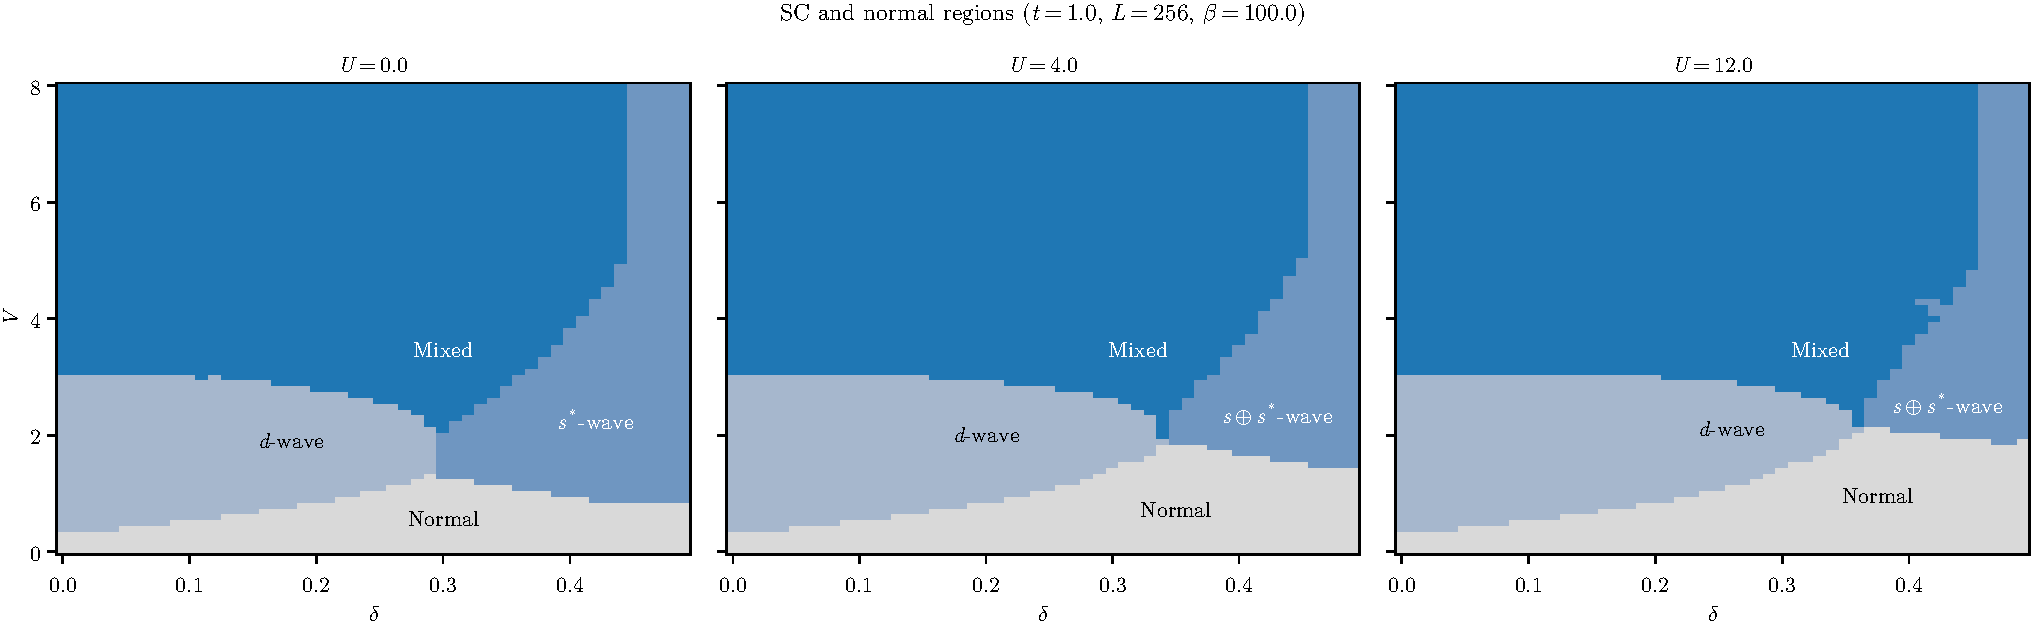
\includegraphics[width=\linewidth]{../Project/src/labs/superconductor-boundary/w-U=[0.0, 4.0, 12.0]-solid.pdf}
	\caption{Depiction of the normal state region and the three singlet superconducting regions, at $U/t=0,4,12$ from left to right. Lighter blue indicates the pure $d$-wave SC phase, blue the isotropic $s \oplus s^*$ phase, deeper blue the mixed region. In text is described the convention we used to identify the boundaries.}
	\label{fig:sc-mix}
\end{figure}

Comparing the three panels of Fig.~\ref{fig:sc-mix}, we see that increasing the value of the local repulsion $U$
the shapes of the four regions change. In particular, the $d$-wave region expands to the right (larger $\delta$s); the normal-$s \oplus s^*$ SC boundary moves up (larger $V$s). Note that on the left panel the isotropic region is labeled as purely $s^*$-wave: this is because if $U=0$, the $s$-wave gap harmonic is null, even if $w^{(s)}$ converges to a non-zero value. The growth of the local repulsion $U$ has two effects:
\begin{enumerate}
	\item turning on the $s$-wave gap harmonic;
	\item expanding the $d$-wave region and restricting the isotropic and mixed region.
\end{enumerate}
From the last point we understand that increasing $U$ we allow for the gap function to have a finite $s$-wave component, but this acts as a sort of internal competition within the isotropic region. Indeed, from the constraint of Eq.~\eqref{eq:sc-wgamma-circle}, we know that $w^{(s)} \neq 0$ only if $w^{(\gamma)} \neq 0$, with $\gamma \neq s$. In the $s \oplus s^*$ region the constraint reads:
\[
	\big| w^{(s^*)} \big|^2 \ge \big| w^{(s)} \big|^2 \frac{U}{V} \, ,
	\qquad
	(\text{Isotropic region})
\] 
Suppose we work at fixed $\delta$ and $V>0$ in the isotropic region at $U=0$. There is no constraint whatsoever on $w^{(s^*)}$. Also, $w^{(s)}$ is free to converge at some finite value (we saw this in the left panel of Fig.~\ref{subfig:sc-data-ws-B256-compared}): the gap still has no $s$-wave component. Suppose now we switch on $U>0$. Now, in order for $w^{(s)}$ to reach the same value as before, $w^{(s^*)}$ has to respect the constraint posed by the above equation. As $U$ increases, the right-hand side gets bigger and $w^{(s^*)}$ needs to converge to larger and larger values to sustain $w^{(s)}$, otherwise to drop to zero. This is why increasing $U$ the isotropic boundary moves up: $w^{(s^*)}$ isn't ``free'' anymore and must respect the constraint of Eq.~\eqref{eq:sc-wgamma-circle}.

In the three panels of Fig.~\ref{fig:sc-mix}, the mixing region is pretty much unchanged. At low doping, it is bounded from below by an horizontal line at $V/t \approx 3$. Increasing doping at fixed $U$, we see that the lower boundary reaches a cusp-like minimum around $\delta \approx 0.3 \divisionsymbol 0.4$ and then grows. This cusp coincides with the aforementioned sharp vertical segment, visible in Fig.~\ref{fig:sc-data-surface-wS-B256}. If we work at fixed doping and $U$, and choose $\delta$ such that we are aligned with the horizontal position of the cusp on the $(\delta,V)$ plane, the critical value of $V/t$ for transitioning to a mixed SC state is minimised. At high values of $V/t$ the mixing region extends to almost unitary doping, being limited on the right by a vertical line at $\delta \gtrsim 0.4$. We remind that we are discerning the SC phases by applying an arbitrary threshold $\varepsilon$ to each gap component: we imagine that by using a more refined technique and by increasing the resolution of the simulation the boundary would appear less straight. Anyway, apart from a vertical stripe at almost unitary filling, at high $V/t$ the dominant singlet SC phase is described by a mix of $d$-wave and $s \oplus s^*$-wave component. Recalling the surface plot of Fig.~\ref{fig:sc-data-surface-wS-B256}, we see that at $V/t \gg 1$ the $s$-wave component gets weaker with respect to the other two. In this limit, if $U \ll V$, the $s$-wave component is negligible, giving an approximate $d \oplus s^*$ mixed phase. 

The mixing region is of particular interest also due its connection with the planar rotational SSB,
\[
	\text{Symmetry mixing}
	\quad\implies\quad
	\mathrm{C}_4 \SSB \mathrm{C}_2 \, .
\]
As we show in next section, the mixed-symmetry region coincides with the portion of the $(\delta,V)$ plane where planar rotational symmetry is broken.

\subsection{Rotational SSB and nematic superconductivity}

In the context of this thesis, nematicity is established whenever $\tilde{t}^{(d)}$ becomes non-zero. This was discussed in detail in the context of the normal phase. If the renormalised hopping parameter has a non-zero $d$-wave component, this means that bare hopping is effectively boosted in one direction and damped in the other. Indeed, from Eq.~\eqref{eq:normal-ud(tx,ty)}, we know that
\[
	\tilde{t}^{(d)} = \frac{\tilde{t}^{(y)} - \tilde{t}^{(x)}}{2} \, .
\]
As we anticipated at the end of Sec.~\ref{subsec:normal-d-wave-hopping}, if $\tilde{t}^{(d)}>0$ the renormalised hopping is larger in direction $y$, if $\tilde{t}^{(d)}<0$ instead it's larger in direction $x$. This interpretation serves to grasp the general idea behind nematicity, but is to be taken carefully. Let us get more rigorous. In the SC phase, the many body state is a gas of Bogoliubov quasiparticles which do not ``hop on neighbouring sites''. If $\tilde{t}^{(d)}$ is non-zero, the superconductor is nematic in the sense that Bogoliubov quasibands are not rotationally invariant,
\[
	\tilde{E}_\mathbf{k} \neq \tilde{E}_{\mathcal{R}\mathbf{k}} \, ,
\]
being $\mathcal{R}$ a $\pi/2$ rotation. We connect this effect to hopping renormalisation \textit{a posteriori} following the formal discussion of Sec.~\ref{subsec:normal-d-wave-hopping}.

\begin{figure}
	\centering
	\subfloat[Dependency of $\tilde{t}^{(d)}$ on $V$ at various $U$s, compared at three values of $\delta$.]{
		
\includegraphics[width=\linewidth]{/home/nepero27178/Thesis/EHM-HF/Project/plots/refined/Mode=hs/Phase=SC-Singlet/Setup=A[256]/Syms=Ssd/RB=Sd/Obj=RMPs/xVar=V_pVar=U/td_t=1.0_L=256_δ=Compared_β=100.0.pdf}
		\label{subfig:sc-data-td-A256-compared}
	}\\
	\subfloat[Dependency of $\tilde{t}^{(d)}$ on $\delta$ at various $V$s, compared at three values of $U$.]{
		
\includegraphics[width=\linewidth]{/home/nepero27178/Thesis/EHM-HF/Project/plots/refined/Mode=hs/Phase=SC-Singlet/Setup=B[256]/Syms=Ssd/RB=Sd/Obj=RMPs/xVar=δ_pVar=V/td_t=1.0_U=Compared_L=256_β=100.0.pdf}
		\label{subfig:sc-data-td-B256-compared}
	}
	\caption{Dependency of the $d$-wave renormalised hopping $t^{(d)}$ varying the doping $\delta$ and the local repulsion $U$. In the top panel we compare three doping levels $\delta=0.0,~0.2,~0.4$ varying $0 \le U \le 8$. In the bottom panel we compare three repulsion values $U=0.0,~5.0,~10.0$ varying $0 \le \delta \le 0.45$.}
	\label{fig:sc-data-td-AB256-compared}
\end{figure}

For the normal and AF phases we were able to prove that $u^{(d)}=0$ for any choice of model parameters. For the SC phase, instead, $u^{(d)}$ converges to non-zero values. For the sake of conciseness, we skip plotting the curves for $u^{(d)}$ {\color{tabred}\textbf{(which are, anyway, openly accessible at our repository)}}, and show directly the curves for the quantity
\[
	\tilde{t}^{(d)} = -\frac{V u^{(d)}}{2} \, .
\]
This is done in Fig.~\ref{fig:sc-data-td-AB256-compared}: nematicity is undoubtedly present. In the top panel (Fig.~\ref{subfig:sc-data-td-A256-compared}), we see that a critical value of $V$ exists over which nematicity is established. Moreover, the $\delta=0.0$ case (left panel) is independent of $U$. In all cases, the convergence values for $\tilde{t}^{(d)}$ are two order of magnitudes smaller than $t=1.0$: in the region of parametric space we explore, nematicity is a sharp but small effect. Note that at $\delta=0.2$ (central panel) $\tilde{t}^{(d)}\ge0$, while at $\delta=0.4$ (right panel) $\tilde{t}^{(d)}\le0$. Increasing the doping we change the sign of $\tilde{t}^{(d)}$

This sign change is most evident in the first two figures of the bottom panel (Fig.~\ref{subfig:sc-data-td-B256-compared}), where we vary the doping level while keeping fixed the local repulsion $U$. The behaviour of $\tilde{t}^{(d)}$ is similar at low doping in the three cases, but changes significantly at larger doping. Indeed, at $U/t=0$ (left figure) and $U/t=5$ (central figure) at some point $\tilde{t}^{(d)}$ changes sign. At $U/t=10$ (right figure), all our data points are positive (possibly the sign flip occurs at higher $V$s). Moreover, as $U$ increases, the amplitude of the oscillation of $\tilde{t}^{(d)}$ as a function of $\delta$ reduces. We conclude that both the local repulsion and electronic doping disrupt nematicity, which is instead most effective for a purely NNs attractive model.

\begin{figure}
	\centering
	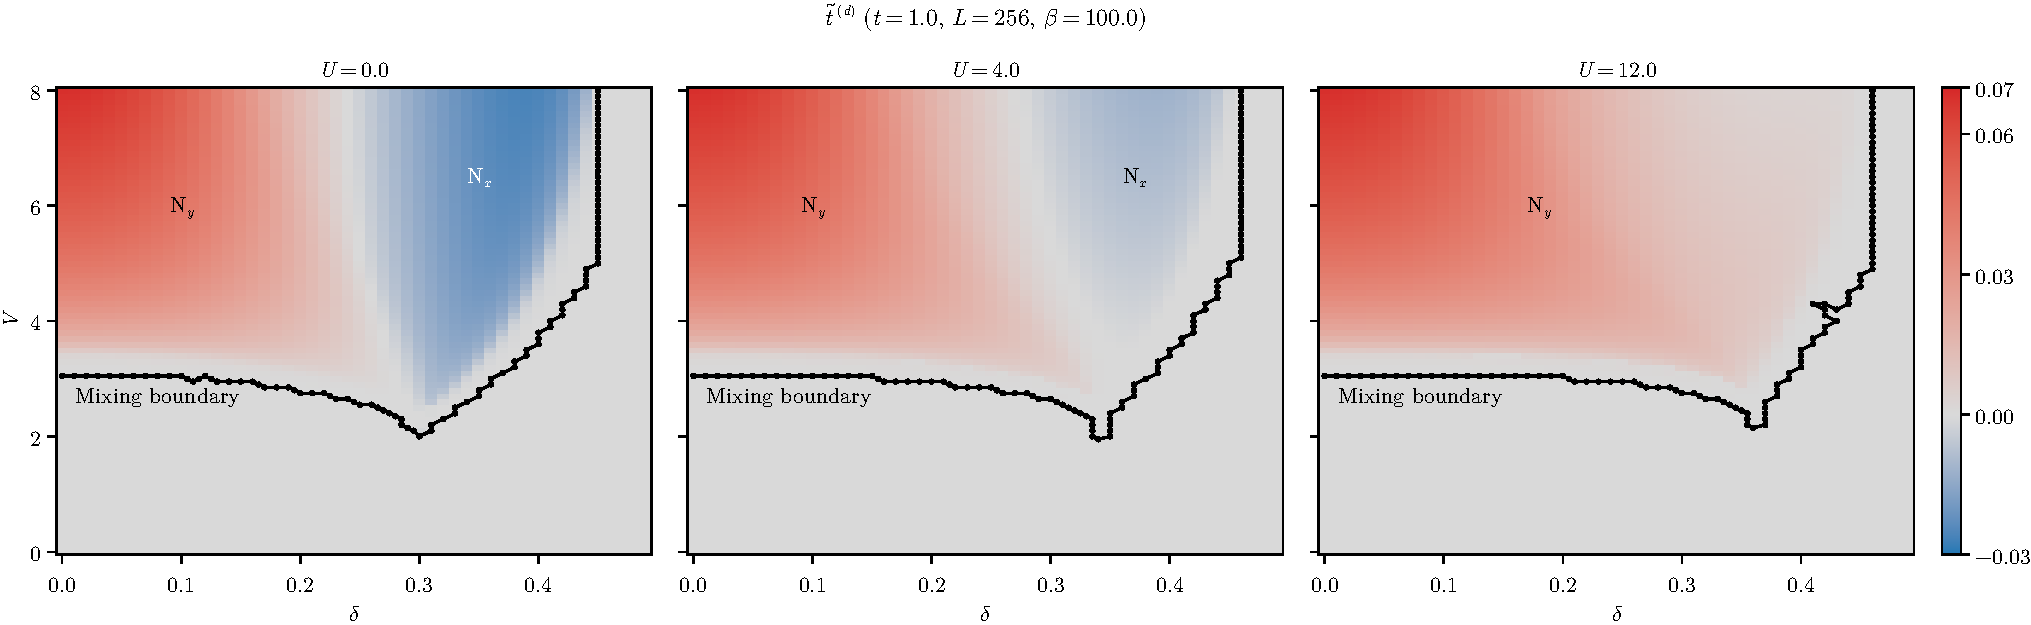
\includegraphics[width=\linewidth]{../Project/src/labs/superconductor-boundary/w-U=[0.0, 4.0, 12.0]-curves.pdf}
	\caption{Heatmap of the anisotropic component of renormalised hopping, $\tilde{t}^{(d)}$, at $U/t=0,4,12$ from left to right. The dataset is the same of Fig.~\ref{fig:sc-mix}, and the mixing boundary is the set of points separating the mixed region from the rest of the phases.}
	\label{fig:sc-td}
\end{figure}

Nematic effects are directly related to symmetry mixing in the superconducting order parameter. Consider Fig.~\ref{fig:sc-td}, where we plot the convergence values for $\tilde{t}^{(d)}$ in the $(\delta,V)$ plane for $U/t=0,4,12$. The used dataset is the same of Fig.~\ref{fig:sc-mix}. The superimposed black lines are the mixing boundaries, the set of extremal points of the deeper blue regions of Fig.~\ref{fig:sc-mix}. Despite a bit of roughness related to the gridded nature of our data, it is evident that these boundaries encircle the regions where $\tilde{t}^{(d)}\neq 0$. Note that the set of points composing the mixing regions are those satisfying the threshold rule exposed in last section; choosing another threshold, the black curves change. Nevertheless, the key point is that there is an evident connection between symmetry mixing and breaking of planar rotational symmetry.

The mixing region coincides with the nematic region. As we said at the beginning of this section, nematicity can be established in two ways, based on the direction along which hopping is boosted. Hence it must hold
\[
	\mathrm{M} \simeq \mathrm{N}_x \cup \mathrm{N}_y
\]
with the following convention on notation:
\[
\begin{aligned}
	\mathrm{M} &= \text{Region of ($\delta,V$) plane where mixing occurs,} \\
	\mathrm{N}_x &= \text{Region of ($\delta,V$) plane where $\tilde{t}^{(d)} < 0$,} \\
	\mathrm{N}_y &= \text{Region of ($\delta,V$) plane where $\tilde{t}^{(d)} > 0$.}
\end{aligned}
\]
The notation $\mathrm{N}_\ell$ has the following meaning: the index $\ell$ indicates the direction along which renormalised hopping is larger. We indicate in Fig.~\ref{fig:sc-td} these regions for $U/t=0,4,12$.

Note that the map were colour-corrected in order to enhance the visibility of the blue region. The intensity of the colouring there suggests that the amplitude is comparable with the red region, but is not. Indeed, we set up the colormap such that gray is aligned with $\tilde{t}^{(d)}=0.0$, and intensity of colour grows asimmetrically in the negative and positive direction.

The three panels of Fig.~\ref{fig:sc-td} differ crucially in the fact that the data for $U/t=12$ (right) are all positive, while those for $U/t=0,4$ (left,centre) are negative in a portion of space. In other words, as we increase $U/t$, $\mathrm{N}_y$ expands and $\mathrm{N}_x$ shrinks. Moving from $U/t=0$ (left) to $U/t=4$ (centre) we see that the amplitude of $\tilde{t}^{(d)}$ decreases in $\mathrm{N}_x$ and not in $\mathrm{N}_y$. We already observed this in Fig.~\ref{subfig:sc-data-td-B256-compared}. Moreover, for $U/t=12$ (right) $\mathrm{N}_x$ is apparently absent and $\mathrm{N}_y$ takes up the entirety of the mixing region. Whether there exists some critical value of $U/t$ above which $\mathrm{N}_x$ disappears in the entirety of the $(\delta,V)$ plane, we do not know.

Breaking of planar rotational symmetry and the insurgence of a $d$-wave harmonic for the renormalised hopping is certainly the most peculiar effect for the singlet SC phase. It adds to the isotropic bands shrinking, which is, the $s^*$-wave renormalisation of the hopping parameter. We discuss it in next section.

\subsection{Isotropic bands shrinking}

\begin{figure}
	\centering
	\subfloat[Dependency of $\tilde{t}^{(s^*)}$ on $V$ at various $U$s, compared at three values of $\delta$.]{
		
\includegraphics[width=\linewidth]{/home/nepero27178/Thesis/EHM-HF/Project/plots/refined/Mode=hs/Phase=SC-Singlet/Setup=A[256]/Syms=Ssd/RB=Sd/Obj=RMPs/xVar=V_pVar=U/tS_t=1.0_L=256_δ=Compared_β=100.0.pdf}
		\label{subfig:sc-data-tS-A256-compared}
	}\\
	\subfloat[Dependency of $\tilde{t}^{(s^*)}$ on $\delta$ at various $V$s, compared at three values of $U$.]{
		
\includegraphics[width=\linewidth]{/home/nepero27178/Thesis/EHM-HF/Project/plots/refined/Mode=hs/Phase=SC-Singlet/Setup=B[256]/Syms=Ssd/RB=Sd/Obj=RMPs/xVar=δ_pVar=V/tS_t=1.0_U=Compared_L=256_β=100.0.pdf}
		\label{subfig:sc-data-tS-B256-compared}
	}
	\caption{Dependency of the $s^*$-wave renormalised hopping $t^{(s^*)}$ varying the doping $\delta$ and the local repulsion $U$. In the top panel we compare three doping levels $\delta=0.0,~0.2,~0.4$ varying $0 \le U \le 8$. In the bottom panel we compare three repulsion values $U=0.0,~5.0,~10.0$ varying $0 \le \delta \le 0.45$.}
	\label{fig:sc-data-tS-AB256-compared}
\end{figure}

The last HFP to be checked is $u^{(s^*)}$, responsible of bands shrinking. Its physical role is the isotropic renormalisation of the hopping parameter
\[
	\tilde{t}^{(s^*)} = t-{V u^{(s^*)}}{2} \, ,
\]
again, we skip plotting $u^{(s^*)}$ and plot directly $\tilde{t}^{(s^*)}$ in Fig.~\ref{fig:sc-data-tS-AB256-compared}. In the top panel (Fig.~\ref{subfig:sc-data-tS-A256-compared}), we show the dependence of $t^{(s^*)}$ on $V$. The three curves, obtained at three doping levels, are approximately independent of $U$. The common feature is that $\tilde{t}^{(s^*)}$ decreases somewhat linearly with $V$ up to some critical value, above which it flattens to an horizontal asymptote. Electronic doping changes primarily the height of this asymptote

As was for the AF and normal phases, electronic doping disrupts the isotropic bands shrinking effect. At half-filling (left figure) we see that bands shrinking is most effective, reducing the hopping parameter to less than half its $V=0$ value. In the bottom panel (Fig.~\ref{subfig:sc-data-tS-B256-compared}) we show $t^{(s^*)}$ as a function of $\delta$, varying $V$ and $U$. As we already noted, the dependence on $U$ is very weak and the three figures are a lot alike. As we already noted, $t^{(s^*)}$ increases with doping.

\begin{figure}
	\centering
	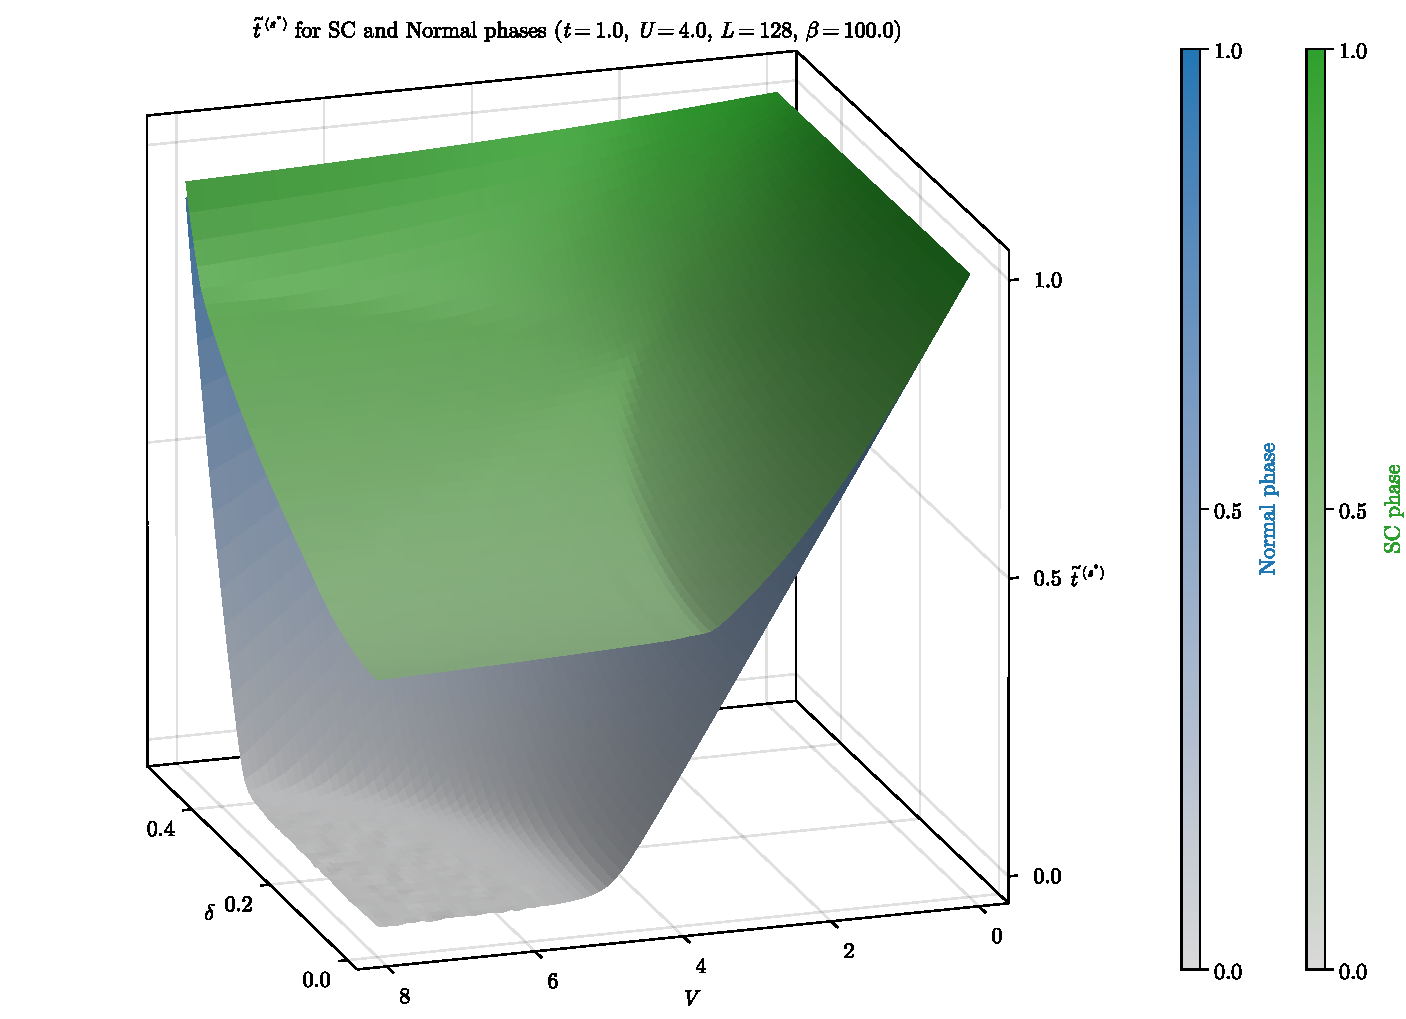
\includegraphics[width=0.7\linewidth]{../Project/src/labs/compare-tS-normal-sc/tS(N)+tS(SC)-ink.pdf}
	\caption{Comparison of the isotropic part of the renormalised hopping $\tilde{t}^{(s^*)}$ for the SC (green) and normal (blue) phases on the $(\delta,V)$ plane. The data from the normal phase are the same of Fig.~\ref{fig:normal-tS-data}.}
	\label{fig:sc-tS-vs-n}
\end{figure}

In Fig.~\ref{fig:sc-tS-vs-n} we compare $t^{(s^*)}$ for the normal phase (blue surface) and the SC phase (green surface). The two surfaces share a general feature: $t^{(s^*)}$ is approximately unitary at low $V/t$ and almost unitary doping, and decreases significantly in the low-$\delta$ and high-$V/t$ limit. In this region, for the normal phase we observe the Mott-localisation plateau discussed in Sec.~\ref{subsec:normal-mott-numeric}, where $t^{(s^*)} \approx 0$. In the SC phase, looking at the same region, $t^{(s^*)}$ is minimised but no plateau is formed. More importantly, isotropic hopping is reduced to roughly half the value of $t$ and not nullified. We do not observe a Mott-like area as for the normal phase.

Recalling the plots of Fig.~\ref{fig:sc-mix}, the low-$\delta$ and high-$V/t$ limit (the corner where $t^{(s^*)}$ is minimised) falls deep within the mixed region. Recalling also Fig.~\ref{fig:sc-data-surface-wS-B256}, in this corner the $d$-wave and $s^*$-wave harmonics of the gap function are large and comparable. Finally, we know from Fig.~\ref{fig:sc-td} (central panel) that here nematic effects are small, but significantly non-zero. In particular, considering that 
\[
	\lim_{\delta \to 0} \lim_{V/t \gg 1} \frac{\tilde{t}^{(s^*)}}{t} \approx 0.4
	\qq{and}
	\lim_{\delta \to 0} \lim_{V/t \gg 1} \frac{\tilde{t}^{(d)}}{t} \approx 0.06 \, ,
\]
we see that the two components differ just by one order of magnitude. Nematic effects account for a rather large portion of hopping renormalisation.

With this consideration, we end the presentation of HFPs and RMPs and move to the last section, where we discuss the results regarding free energy and entropy densities.

\subsection{Solution free energy and entropy densities}\label{subsec:sc-f-s}

\begin{figure}
	\centering
	
\includegraphics[height=0.32\linewidth]{/home/nepero27178/Thesis/EHM-HF/Project/src/labs/superconductor-plot-fs/fs_U=4.0.pdf}
	\caption{Heatmaps of the free energy and entropy densities at $U/t=4$. The black dotted lines represent the internal boundaries of the singlet SC phase, extracted from Fig.~\ref{fig:sc-mix}.}
	\label{fig:sc-data-fs-B128}
\end{figure}

For the SC phase, free energy density is given by Eq.~\eqref{eq:sc-fMFT}, while entropy density is given by Eq.~\eqref{eq:sc-s}. In Fig.~\ref{fig:sc-data-fs-B128} we plot, sided, the heatmaps for $f$ and $s$ at $U/t=4$ in the $(\delta,V)$ plane. Superimposed, we show the boundaries between the four regions identified in Fig.~\ref{fig:sc-mix}. Consider first the free energy, on the left: our data suggest that free energy is maximised in the $d$-wave phase, followed by the mixed phase. At high doping, the $s \oplus s^*$-wave phase is low-energetic. Overall, $f$ varies smoothly across phase boundaries, and we do not identify the black lines with some isoenergetic line separating phases.

This is not the case for entropy density. Indeed, the entropic region on the right panel of Fig.~\ref{fig:sc-data-fs-B128} coincides with the normal phase. The three superconducting regions are low-entropic. This is explained by the following argument:
\begin{itemize}
	\item In the normal phase, the Bogoliubov band reduces to $\tilde{E}_\mathbf{k} \to \tilde{\xi}_\mathbf{k}$. The chemical potential crosses the bare band and a Fermi surface exists. Hence, at finite temperature, the Fermi-Dirac occupation of single-particle states varies continuously from almost unitary (deep in the Fermi sea) to almost zero (far outside). All those states in the middle, around the Fermi level, are highly entropic: we have shown this in Fig.~\ref{subfig:normal-entropy}. It  is the intrinsic metallic nature of the normal phase that makes is entropic.
	\item In the SC phase, we open a gap at the chemical potential, not at zero energy (as instead was in the AF phase). Computing entropy as in Sec.~\ref{subsec:sc-s}, we apply the Fermi-Dirac distribution on the two bands $\pm\tilde{E}_\mathbf{k}$. As the gap opens, the lower one fills ($f \approx 1$), while the upper empties ($f \approx 0$). As we lower temperature, the above statement gets exact. Recalling Fig.~\ref{subfig:normal-entropy}, we see that entropy is minimised at $f=0,1$. Hence, the SC phase is low-entropic.
\end{itemize}
This is the reason behind the sharp separation of the normal region from the SC regions in the right panel of Fig.~\ref{fig:sc-data-fs-B128}.

\begin{figure}
	\centering
	\subfloat[Dependency of $f$ on $V$ at various $\delta$s, compared at three values of $U$.]{
		
\includegraphics[width=\linewidth]{/home/nepero27178/Thesis/EHM-HF/Project/plots/refined/Mode=hs/Phase=SC-Singlet/Setup=B[256]/Syms=Ssd/RB=Sd/Obj=phys/xVar=V_pVar=δ/f_t=1.0_U=Compared_L=256_β=100.0.pdf}
		\label{subfig:sc-data-f-B256-compared}
	}\\
	\subfloat[Dependency of $s$ on $V$ at various $\delta$s, compared at three values of $U$.]{
		
\includegraphics[width=\linewidth]{/home/nepero27178/Thesis/EHM-HF/Project/plots/refined/Mode=hs/Phase=SC-Singlet/Setup=B[256]/Syms=Ssd/RB=Sd/Obj=phys/xVar=V_pVar=δ/s_t=1.0_U=Compared_L=256_β=100.0.pdf}
		\label{subfig:sc-data-s-B256-compared}
	}
	\caption{Dependency of free energy (top) and entropy (bottom) densities on $V$ varying the doping $\delta$ and the local repulsion $U$.}
	\label{fig:sc-data-fs-B256-compared}
\end{figure}

In Fig.~\ref{fig:sc-data-fs-B256-compared} we show $f$ and $s$ as functions of $V$, varying $\delta$ and comparing for three values of $U$. On both rows, moving from left to right we do not observe significant differences: $f$ and $s$ depend weakly on $U$. We already observed the presence of a maximum of the free energy at ratios $V/t$ comparable with $1$. In Fig.~\ref{subfig:sc-data-f-B256-compared} we see this maximum around $V/t \lesssim 4$. Comparing with the data of Fig.~\ref{fig:sc-data-fs-B128}, we can imagine that this maximum could be located at at the boundary between $d$-wave and mixed regions. Our data and methods are too rough to assert with certainty.

In the bottom panel, entropy density (Fig.~\ref{subfig:sc-data-s-B256-compared}) shows the aforementioned sharp separation between normal and SC regions, and is maximised at half-filling and $V=0$. That is the case of the conventional HM. We already argued that superconductivity is impossible at HF level, while commensurate antiferromagnetism is favoured at null doping with respect to the normal phase.

\begin{figure}
	\centering
	\subfloat[Energy difference with normal phase.]{
		
\includegraphics[width=0.45\linewidth]{/home/nepero27178/Thesis/EHM-HF/Project/src/labs/compare-f-normal-sc/f(N)-f(SC)-ink.pdf}
		\label{subfig:sc-Δf-n}
	}
	\subfloat[Energy difference with AF phase.]{
		
\includegraphics[width=0.45\linewidth]{/home/nepero27178/Thesis/EHM-HF/Project/src/labs/compare-f-af-sc/f(AF)-f(SC)-ink.pdf}
		\label{subfig:sc-Δf-af}
	}
	\caption{Surface plots of the energies among the three phases. For the normal phase, we use that fact that $f^{(\mathrm{SC})}$ depends weakly on $U$, while $f^{(\mathrm{N})}$ does not depend on it at all, to limit to the case $U/t=4$. For the AF phase, we limit to the half-filling condition and show data in the $(U,V)$ plane.}
	\label{fig:sc-Δf}
\end{figure}

To conclude, we compare the free energy of the SC phase with that of the normal phase and the AF phase. We said that $f$ depends rather weakly on $U$ for the singlet SC phase, so we carry out the comparison with normal phase at $U/t=4$ in the $(\delta,V)$ plane. In Fig.~\ref{subfig:sc-Δf-n} we plot the quantity
\[
	f^{(\mathrm{N})} - f^{(\mathrm{SC})} \, ,
\]
and observe that it is greater or equal to zero over the entire explored region. The energy difference is null only at $V/t \lesssim 2$, where the superconducting gap is null. We plot, superimposed, the boundaries of the normal region extracted from Fig.~\ref{fig:sc-mix}. In the rest of the $(\delta,V)$ plane the SC phase is energetically favoured with respect to the normal phase. 

In Fig.~\ref{subfig:sc-Δf-af} we show the energy difference between AF and SC phases,
\[
	f^{(\mathrm{AF})} - f^{(\mathrm{SC})} \, .
\]
We colour-corrected the surface plot to align the gray with the $f=0$ level. Colour separates positive and negative regions: the SC phase is dominant where $f^{(\mathrm{AF})} > f^{(\mathrm{SC})}$ (green region), in the rest of the plot the AF phase dominates (blue region). We indicate the contour level at $f=0$ as a black dotted line, obtained as the set of data points whose energy difference is closest to zero. At half-filling, commensurate antiferromagnetism is almost everywhere energetically favoured. Singlet superconductivity prevails in the $U/t \ll 1$, $V/t \gg 1$ limit. The fact that the phase boundary has somewhat a linear shape suggests the fact that possibly a critical ratio exists,
\[
	\left(\frac{V}{U}\right)_\mathrm{c} = k \, ,
	\qquad
	\text{(Critical ratio)}
\]
delimiting a phase transition from antiferromagnetic to superconducting ordering at half-filling.

\section{A final note}

We conclude this chapter with a note of method. We performed simulations on the singlet channel, but also gathered data for the triplet channel. We omitted to show them in order to avoid unnecessary complications. Indeed, we observed that triplet superconductivity (as we formulated it at HF level) is suppressed everywhere in the region of parametric space we are exploring. This means that 
\[
	w^{(p_x)} = w^{(p_y)} = 0 \, .
	\qquad
	\text{(Observed numerically)}
\]
Although non present in this discussions, {\color{tabred}\textbf{the plots for these HFPs are openly accessible at our repository.}}

We did not provide any theoretical constraint on the five HFPs for the singlet SC phase. We tried to obtain a proof similar to those presented for the normal and AF phases, but we did not find any. It would be interesting, if possible, to work out a method to express analytically the position of the various boundaries we identified.